
\section{Scalability Campaign}\label{results:scale}

Given the base parameter values described in Tables \ref{tbl:front_ref_params}
and \ref{tbl:back_ref_params}, exchanges were generated by scaling the number of
reactors in the system. The smallest system modeled included five reactors. The
largest exchanges included five-hundred reactors, a value chosen because there
are approximately five-hundred reactors currently operating (437) or under
construction (71) in the world \cite{nrxtrs}. Therefore, the largest exchanges
modeled represent a time step in a simulation in which the world-wide fleet of
reactors are all supplying or consuming a batch of fuel.

Front and back-end exchanges are explored similarly in the scalability
campaign. First, for all 18 combinations of fundamental parameters and each
solver, a set of reference cases are established, where the only varying
parameter is the number of reactors. Next, specific instance parameters are
chosen to vary in order to determine first-order effects as the exchange system
size scales. Finally, the effect of convergence criteria for the CBC solver is
investigated.

Individual figures for each experiment are provided for each fuel cycle modeled
($f_\text{fc}$) and each solver. Each figure summarizes the results for all
combinations of $f_\text{rx}$ and $f_\text{loc}$. The layout for each six-pane
figure is shown below.

\begin{figure}[h!]
  \begin{center}
    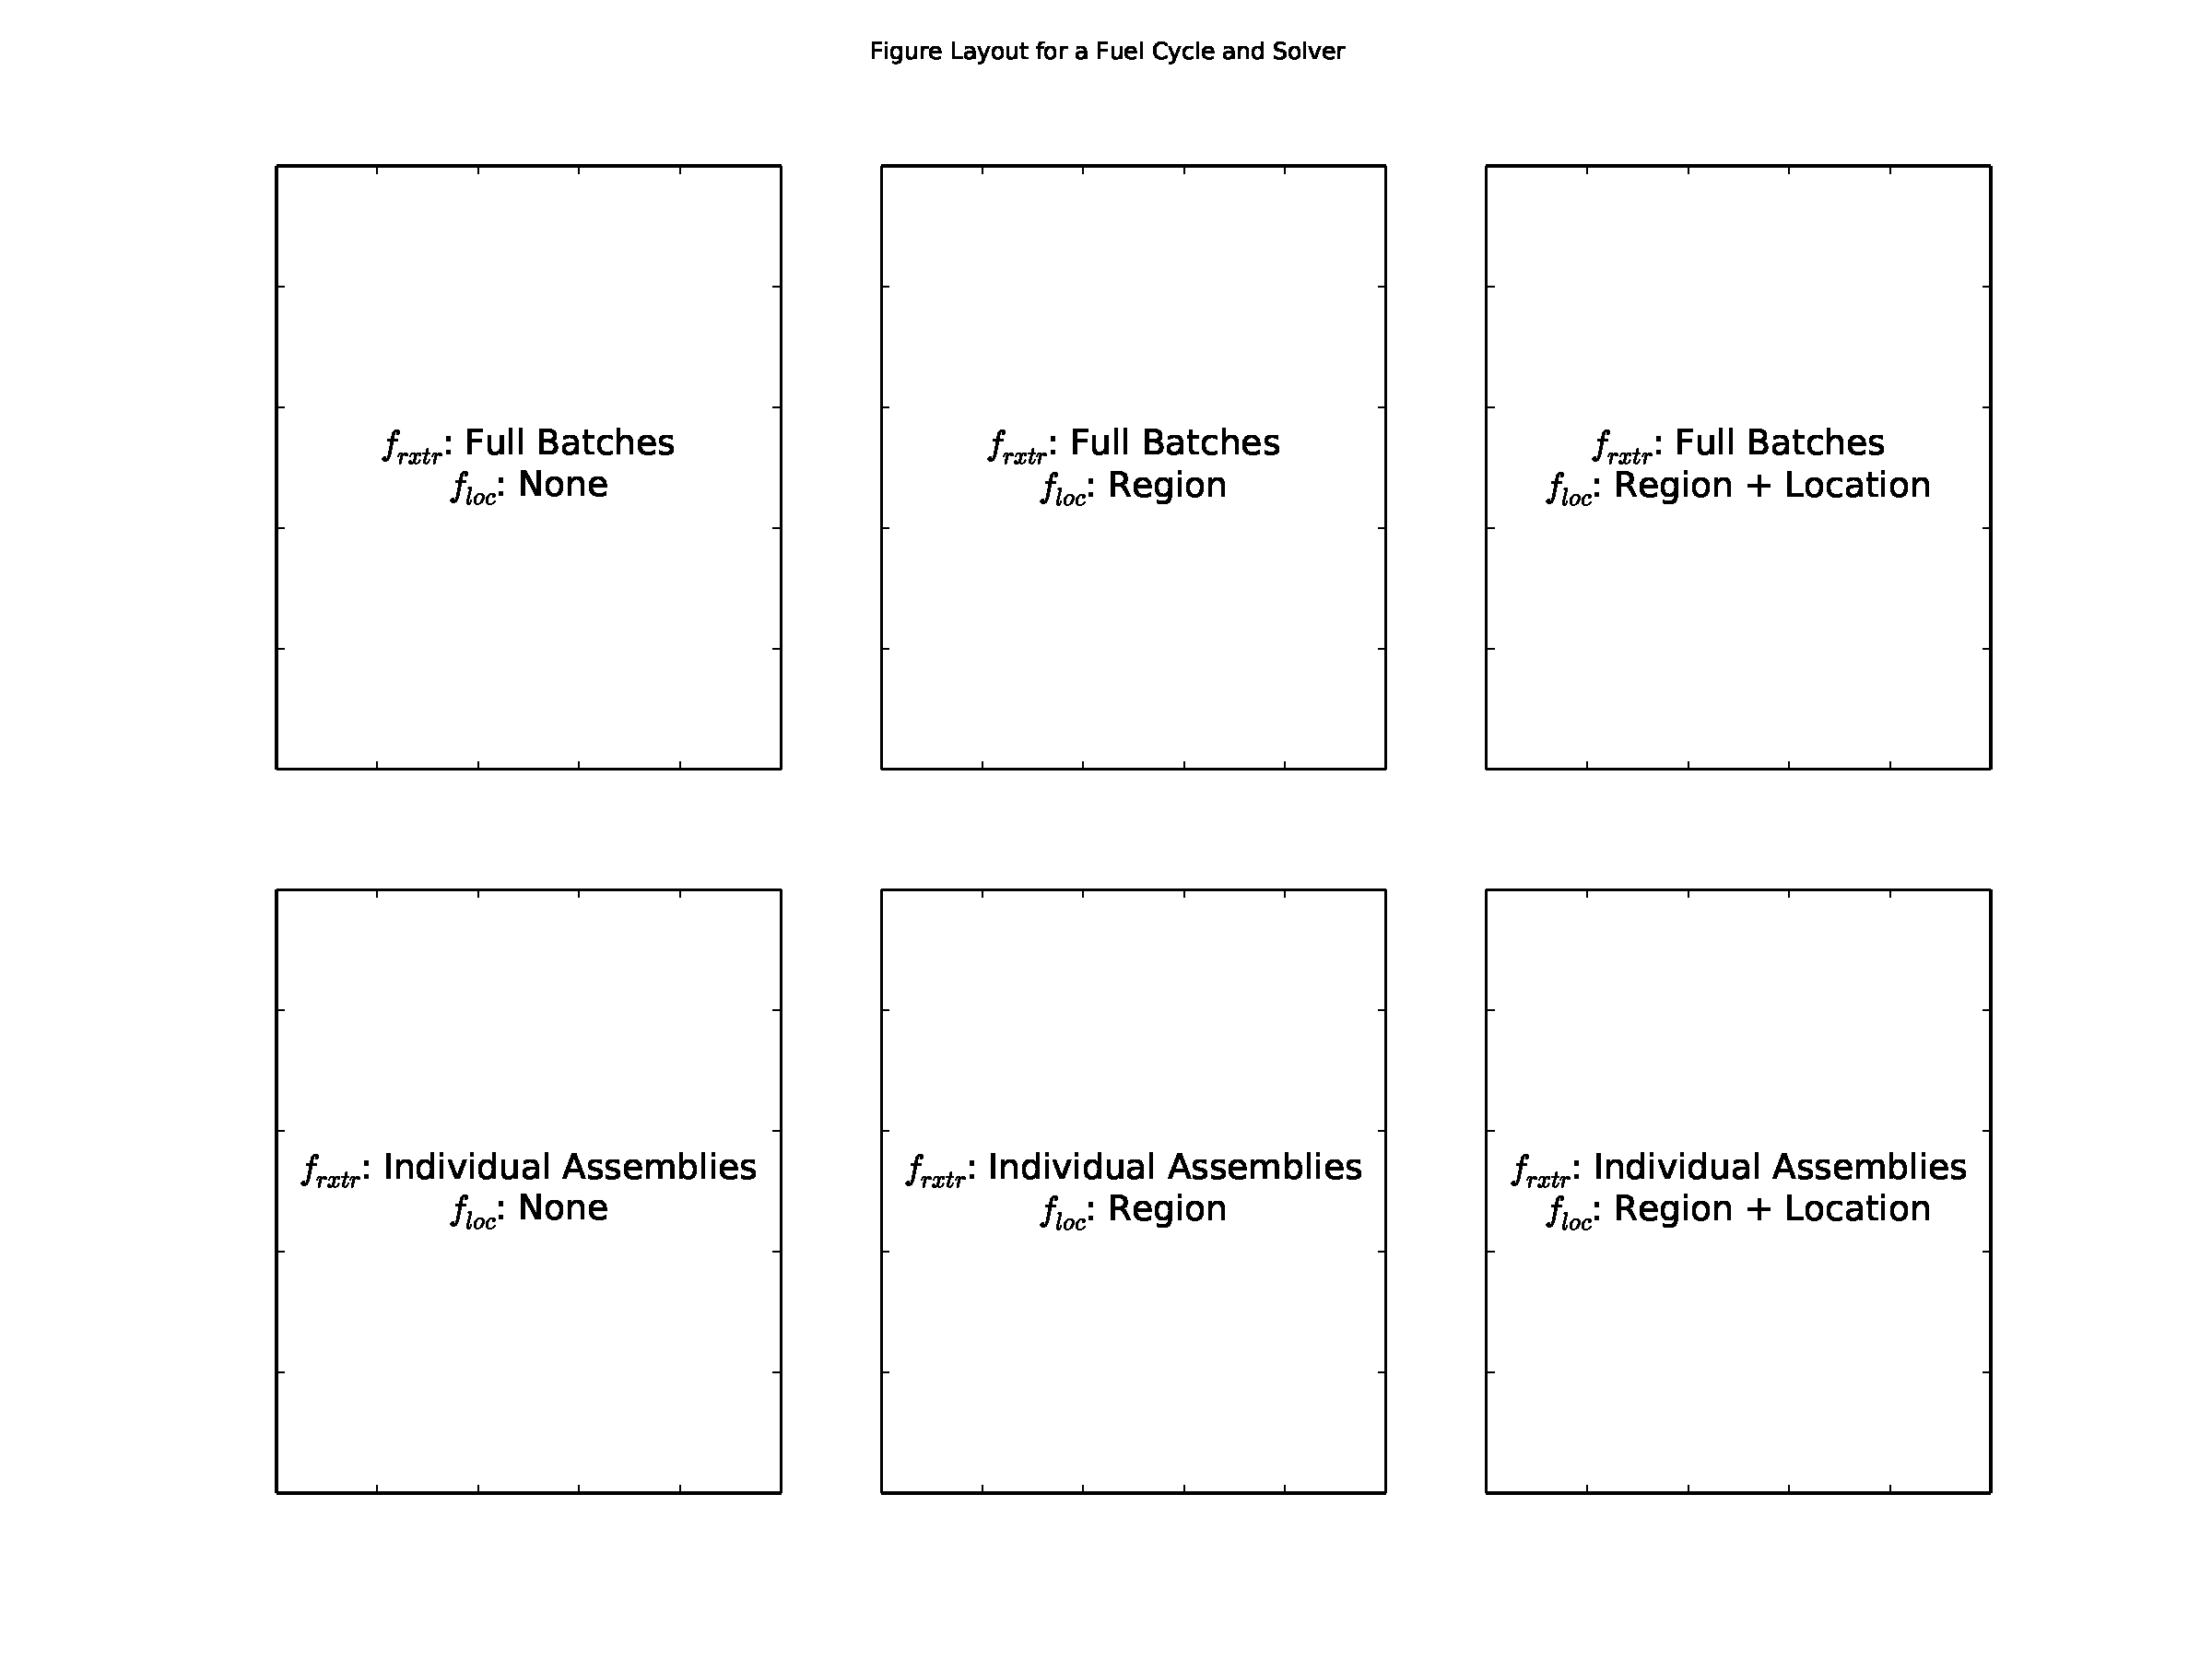
\includegraphics[width=.7\textwidth]{figure_layout.pdf}
    \caption[]{
      \label{fig:figure_layout}
      The general figure layout displaying results for different fundamental
      parameter values.}
  \end{center}
\end{figure}

\subsection{Front-End Exchanges}

\subsubsection{Reference Case}

Reference cases were generated for front-end exchanges by scaling the number of
reactors in each exchange. A step size of 5 reactors was used for the range of
$[5, 100]$ and a step size of 25 was used from $(100, 500]$. In mathematical
  programming, the number of variables and number of constraints in a problem
  are measures of problem scaling. In the NFCTP, constraints are provided by
  trading entities, and the number of variables is equal to the number of arcs
  in a given exchange graph. Accordingly, understanding how each quantity scales
  with the number of reactors is of chief import.

Figure \ref{fig:base_front_n_rxtr_n_arcs_fc1_greedy} shows how the number
of arcs scale with problem size for the MOX fuel cycle, and Figure
\ref{fig:base_front_n_rxtr_n_constrs_fc1_greedy} shows the same results
for the number of constraints. The number of constraints scales linearly, for it
is a purely function of the number of entities in an exchange. However, the
number of arcs scales by $\mathcal{O}(n^2)$. During exchange generation, the
number of suppliers is a function of the number of reactors. Further, each
reactor and each supplier have an arc connecting them if the reactor can consume
the supplier's commodity. Therefore, adding a single reactor to the system
results in additional arcs for every reactor previously existing in the system,
resulting in an $\mathcal{O}(n^2)$ relationship. Both relationships hold true
regardless of the fuel cycle being modeled, and, as can be seen, are also
independent of other fundamental parameters. The arc population magnitude,
however, is a function of $f_\text{rxtr}$. As $f_\text{rxtr}$ increases, $n_a$
individual assemblies are requested rather than a single batch.

\begin{figure}[h!]
  \begin{center}
    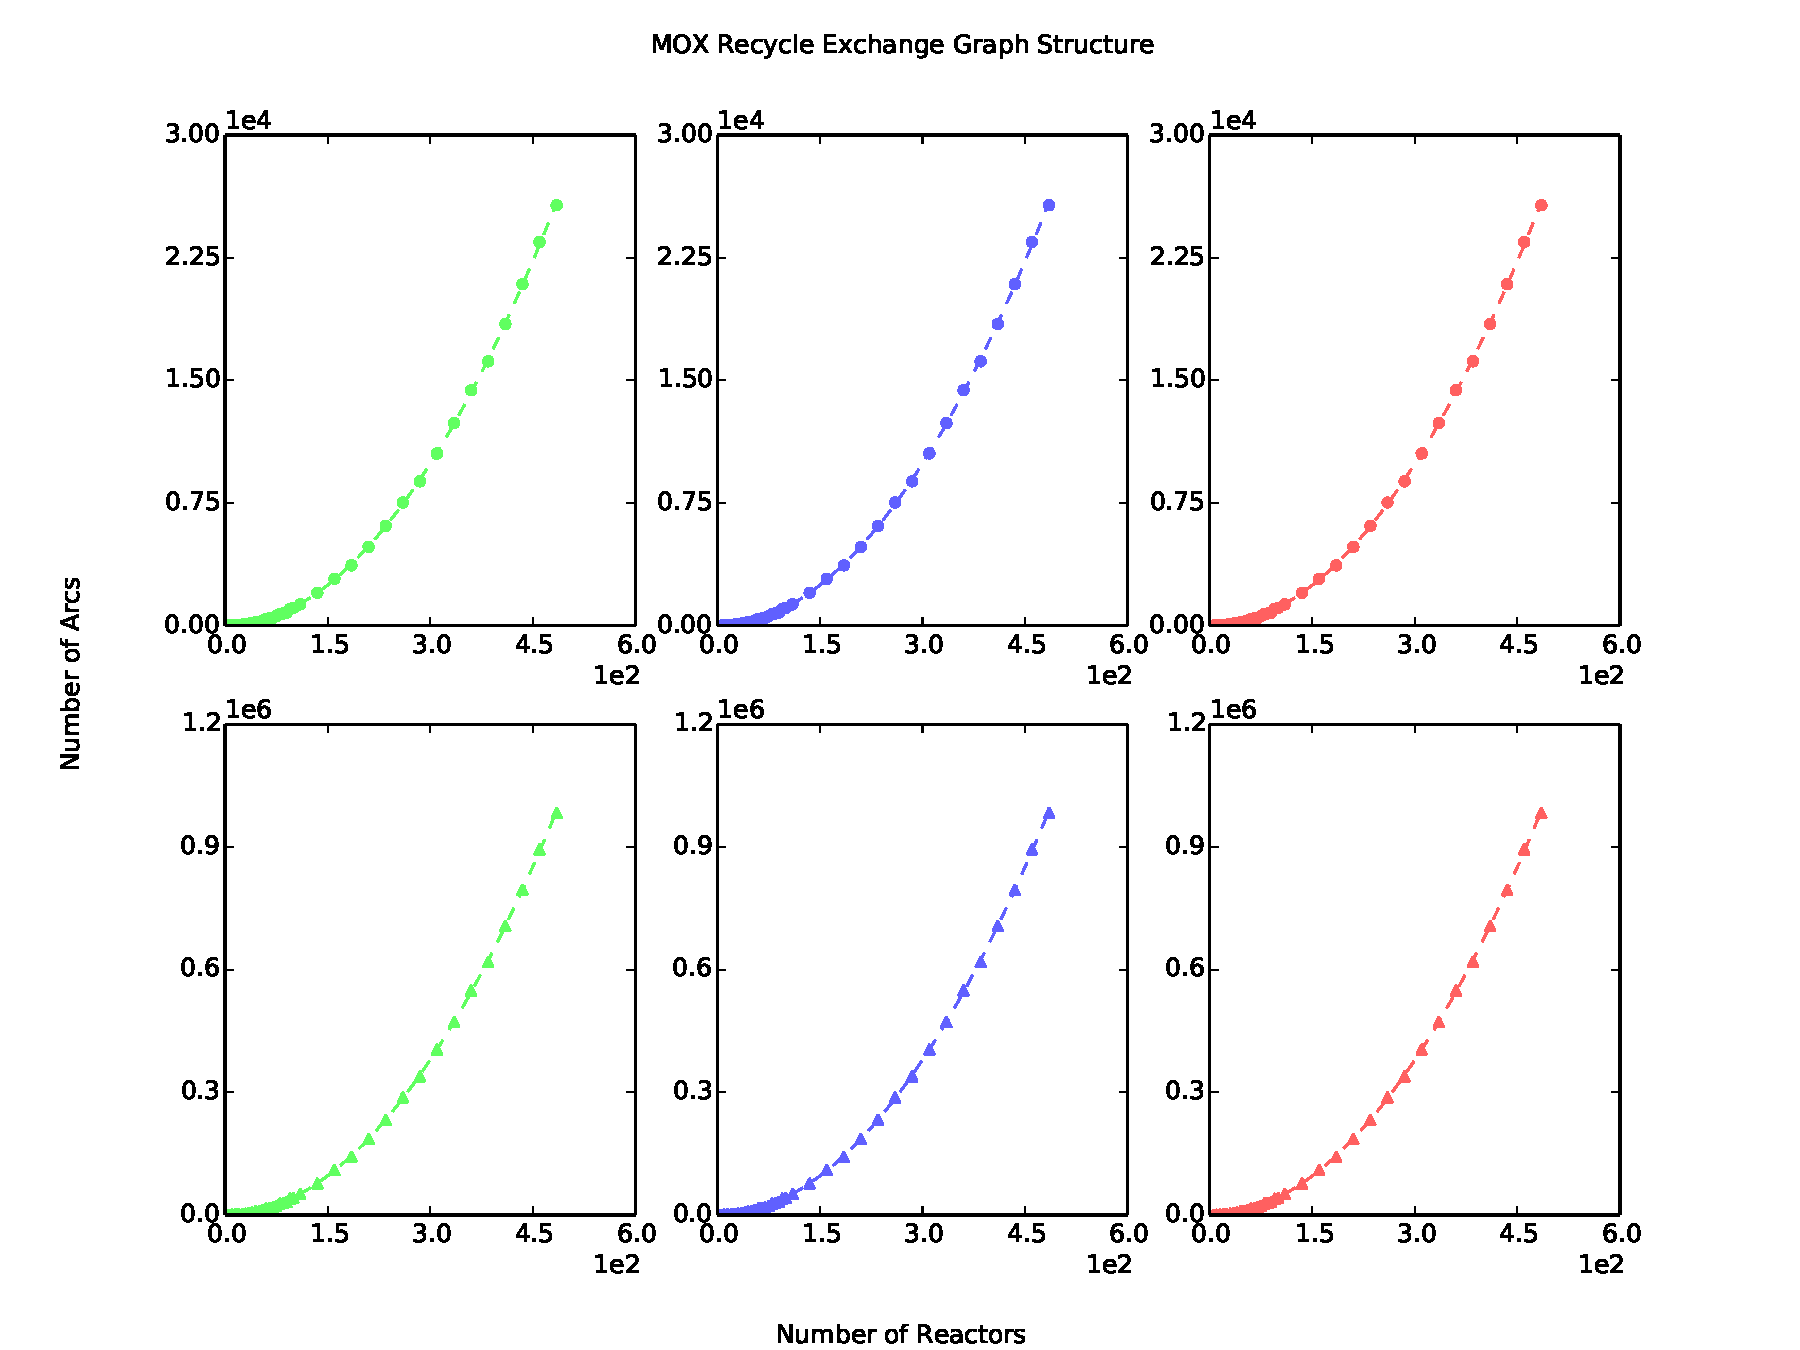
\includegraphics[width=.7\textwidth]{base_front_n_rxtr_n_arcs_fc1_greedy.pdf}
    \caption[]{
      \label{fig:base_front_n_rxtr_n_arcs_fc1_greedy}
      Arc population scaling with the number of reactors with corresponding
      quadratic fits.}
  \end{center}
\end{figure}

\begin{figure}[h!]
  \begin{center}
    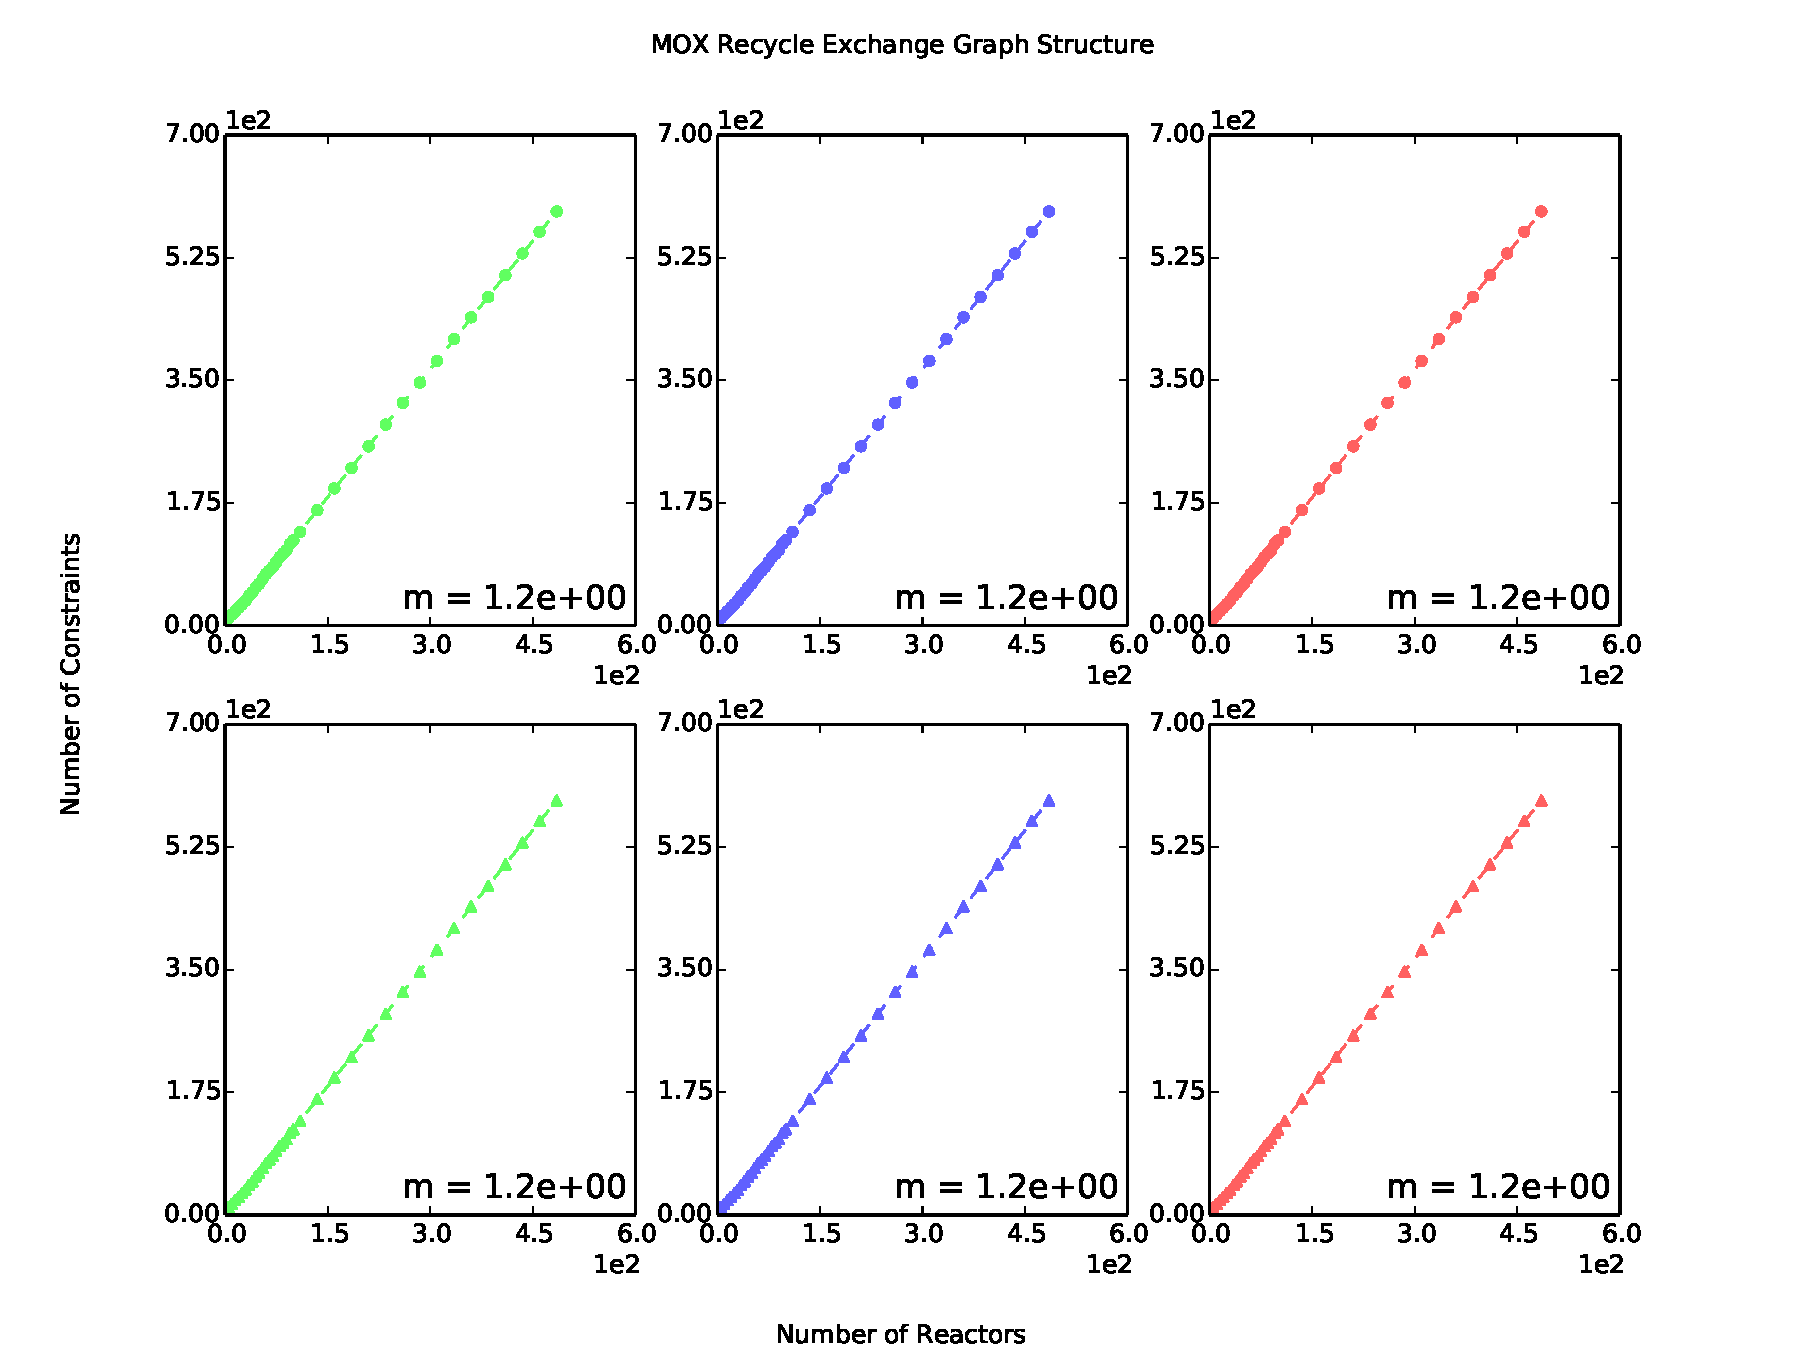
\includegraphics[width=.7\textwidth]{base_front_n_rxtr_n_constrs_fc1_greedy.pdf}
    \caption[]{
      \label{fig:base_front_n_rxtr_n_constrs_fc1_greedy}
      Constraint population scaling with the number of reactors with
      corresponding linear fits.}
  \end{center}
\end{figure}

\paragraph{Greedy Solver}

\cref{fig:base_front_n_arcs_time_fc0_greedy,fig:base_front_n_arcs_time_fc1_greedy,fig:base_front_n_arcs_time_fc2_greedy}
show the Greedy Solver results as the number of arcs increases for the OT, MOX,
and ThOX fuel cycles, respectively. Plotted with each data set is a linear fit
with associated slope value. As expected, the algorithm scales as
$\mathcal{O}(n)$ with the number of arcs in the system. This scaling behavior is
consistent across all fundamental parameters. Of note, however, is that the
scaling constant does increase when moving from low-fidelity reactor models to
higher-fidelity models.

\begin{figure}[h!]
  \begin{center}
    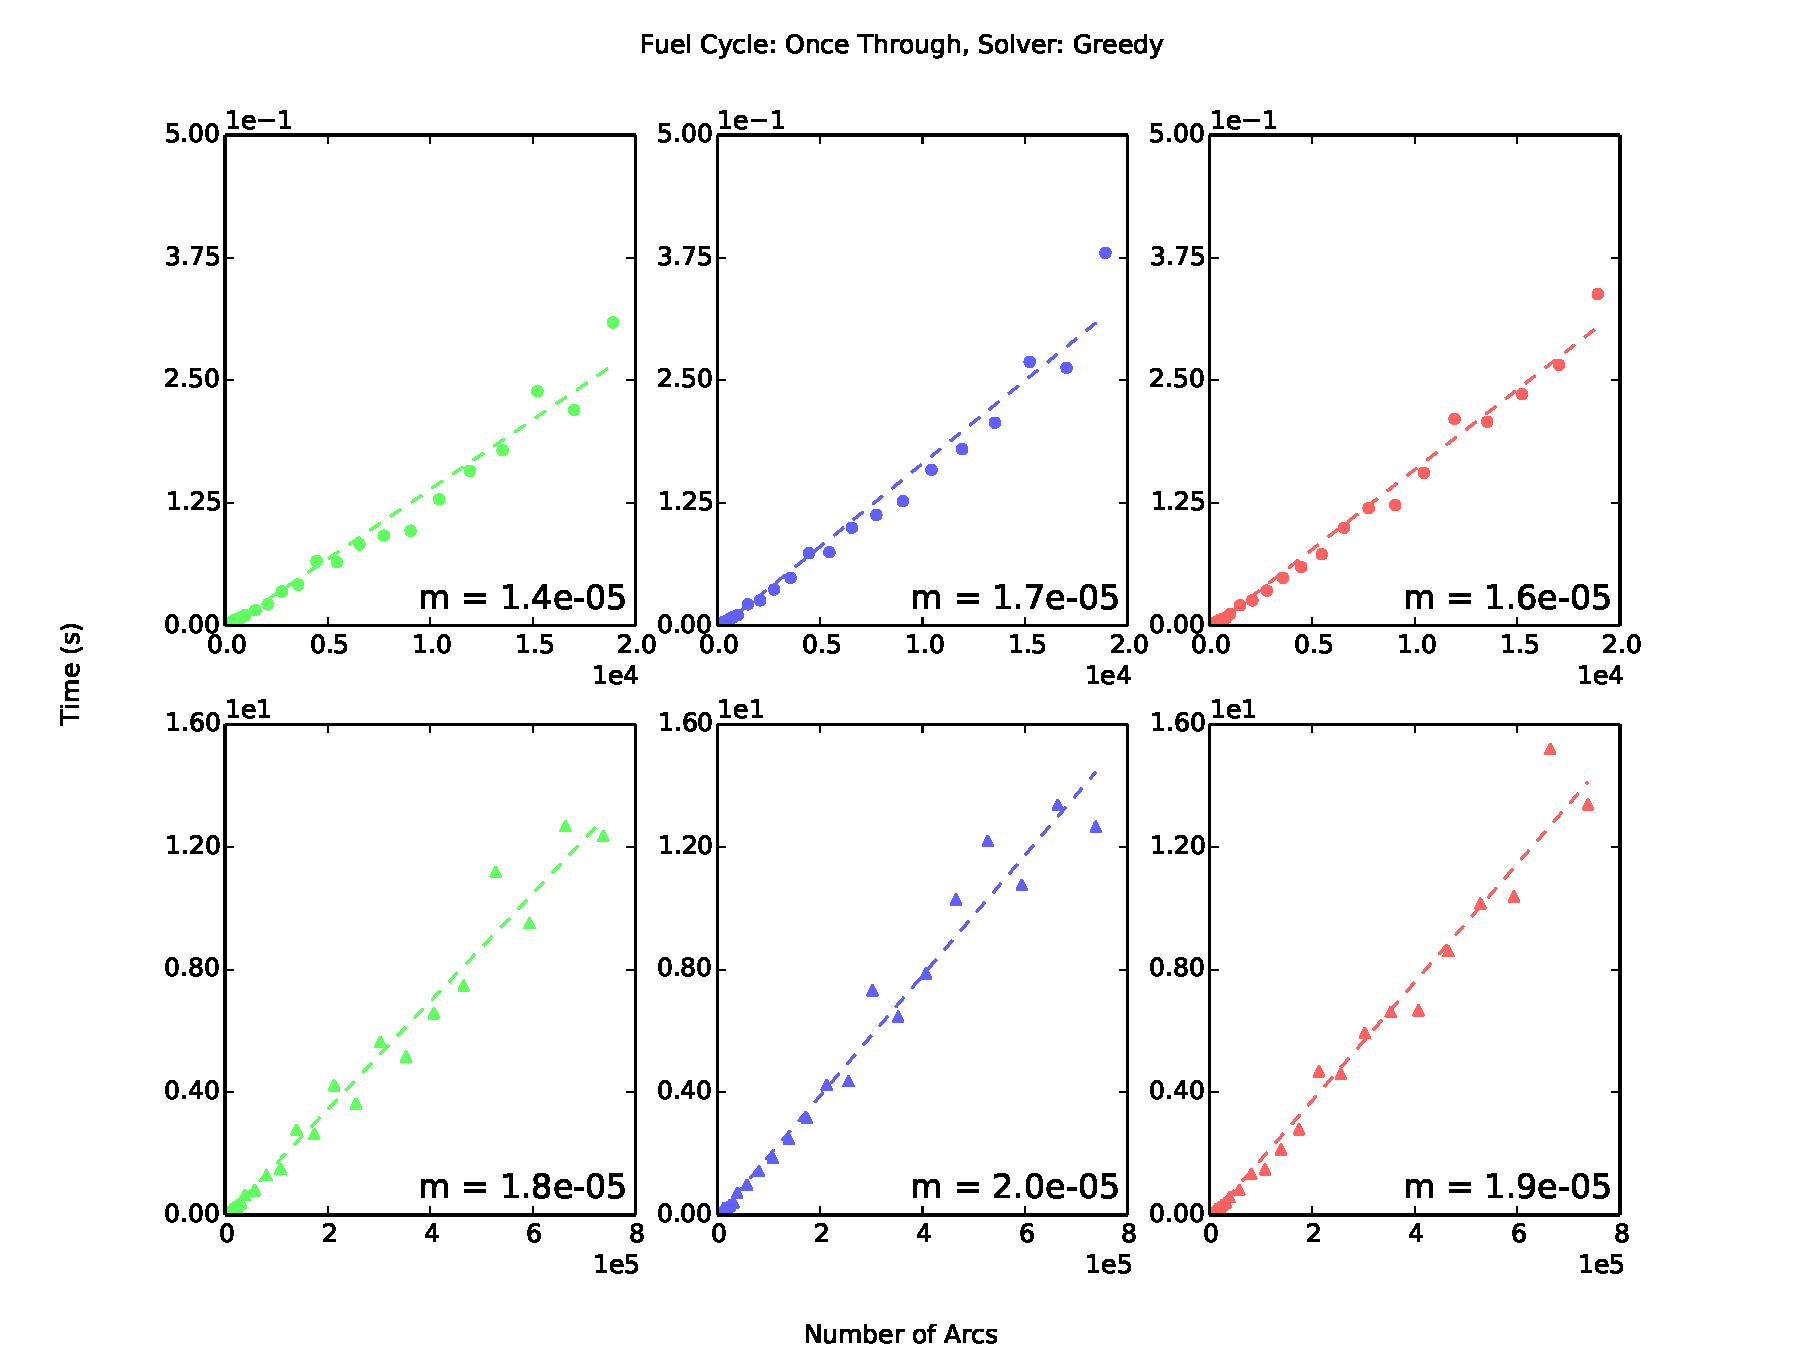
\includegraphics[width=.7\textwidth]{base_front_n_arcs_time_fc0_greedy.pdf}
    \caption[]{
      \label{fig:base_front_n_arcs_time_fc0_greedy}
      Greedy Solver results for the OT fuel cycle as the number of arcs
      increases.  }
  \end{center}
\end{figure}

\begin{figure}[h!]
  \begin{center}
    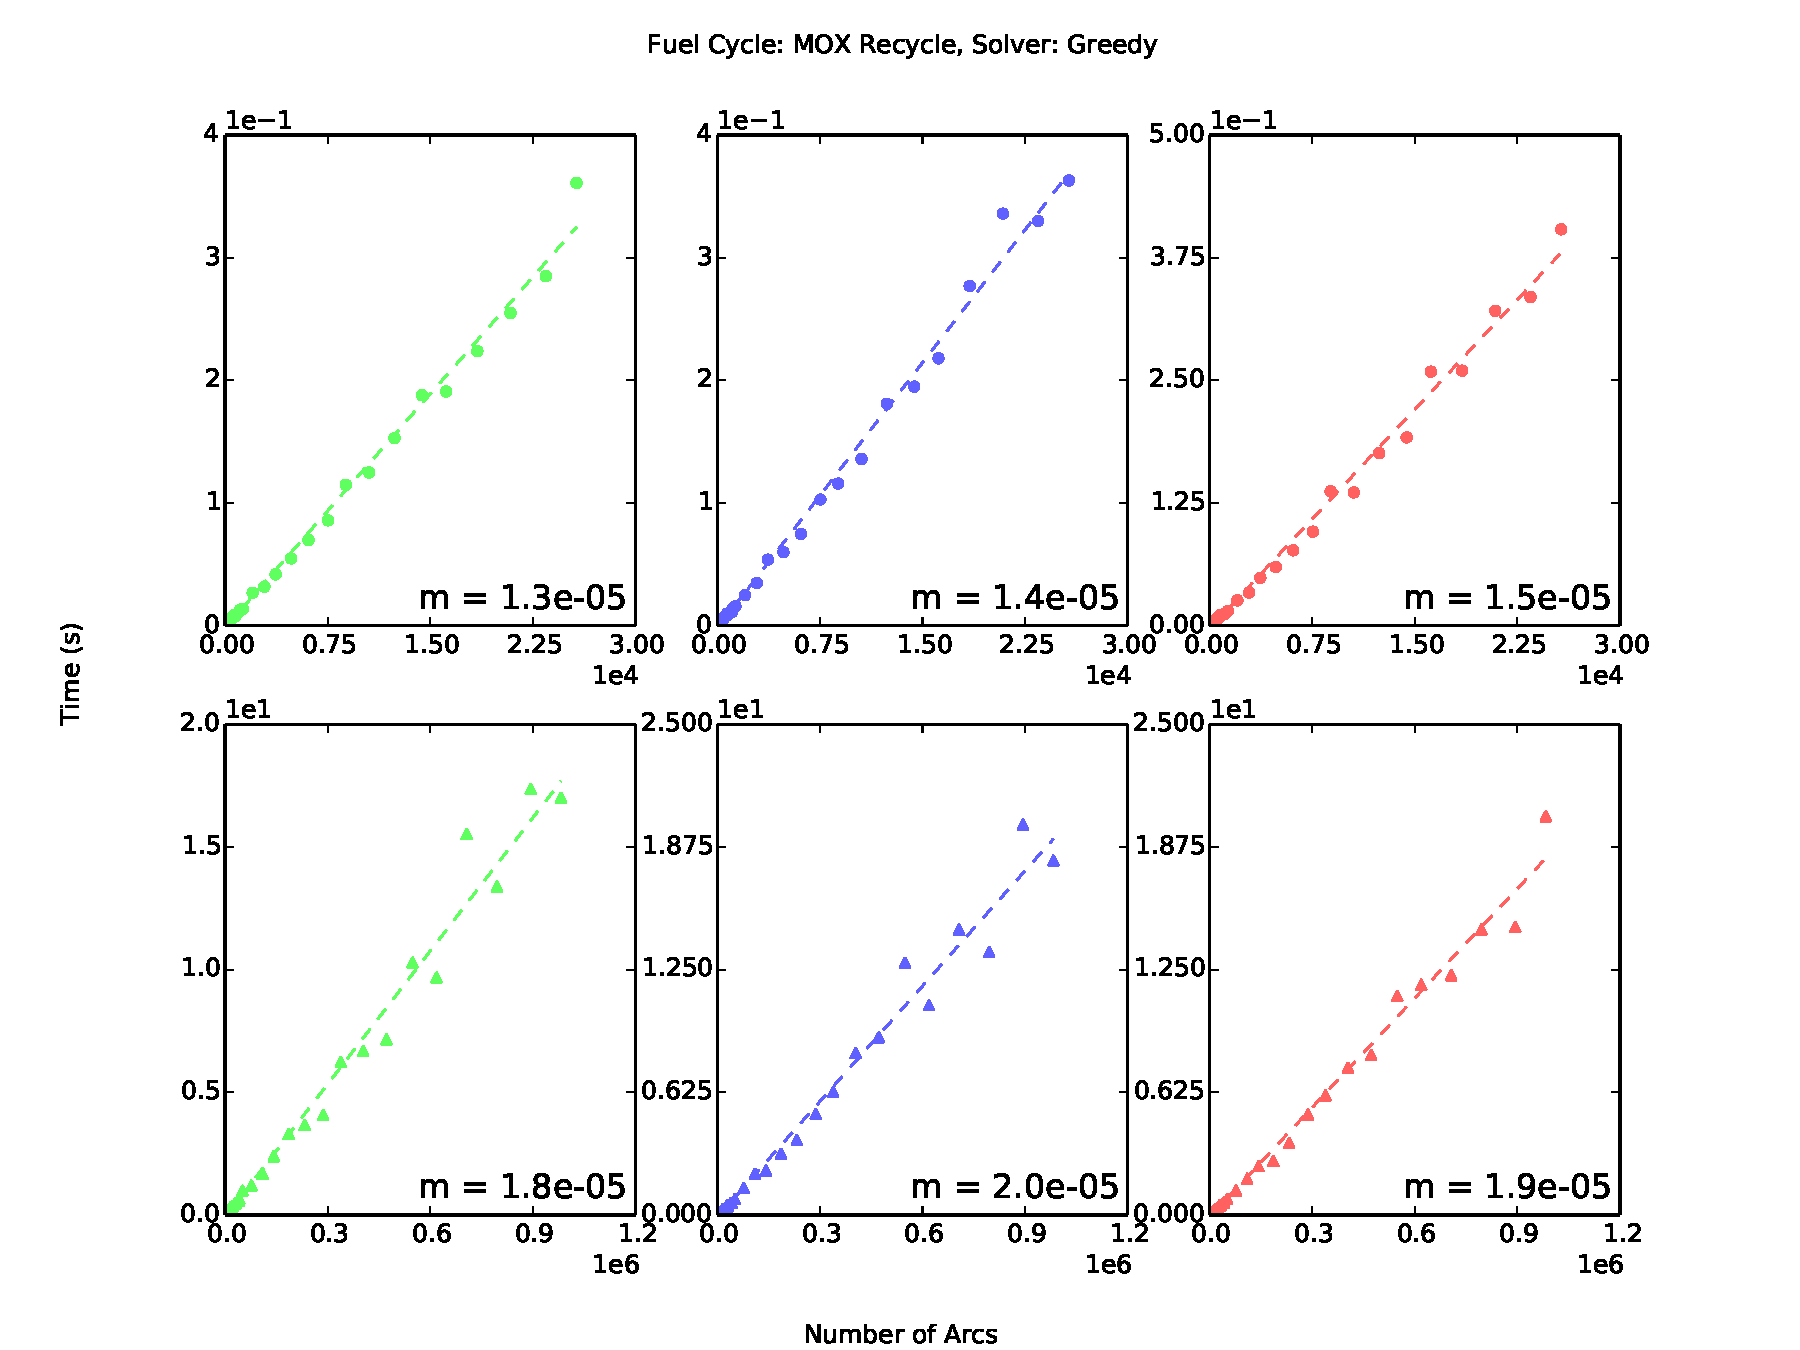
\includegraphics[width=.7\textwidth]{base_front_n_arcs_time_fc1_greedy.pdf}
    \caption[]{
      \label{fig:base_front_n_arcs_time_fc1_greedy}
      Greedy Solver results for the MOX fuel cycle as the number of arcs
      increases.
    }
  \end{center}
\end{figure}

\begin{figure}[h!]
  \begin{center}
    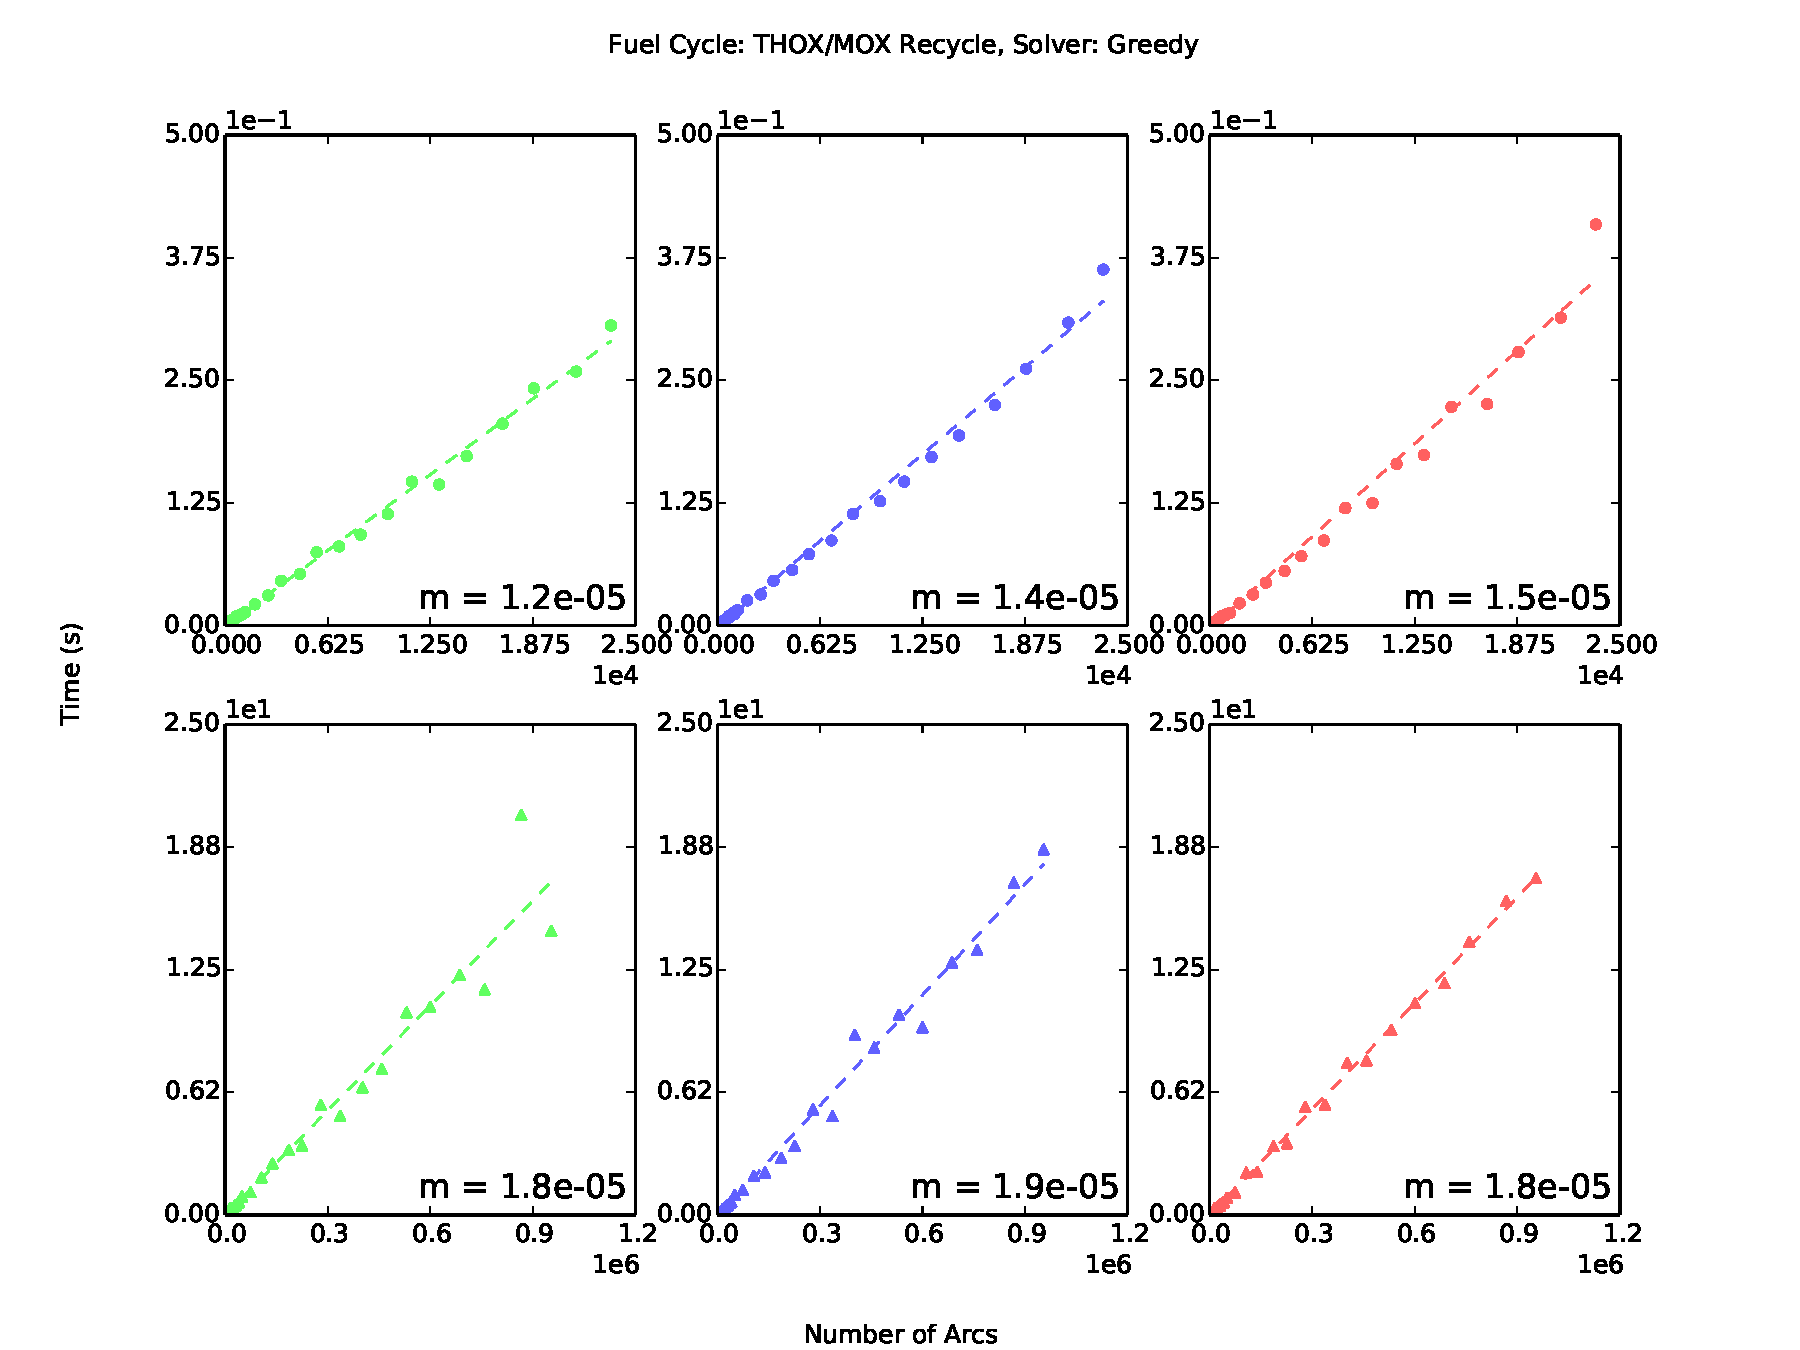
\includegraphics[width=.7\textwidth]{base_front_n_arcs_time_fc2_greedy.pdf}
    \caption[]{
      \label{fig:base_front_n_arcs_time_fc2_greedy}
      Greedy Solver results for the ThOX fuel cycle as the number of arcs
      increases.
      }
  \end{center}
\end{figure}

\paragraph{CLP Solver}

Interestingly, the CLP solver shows the similar scaling behavior as the Greedy
Solver, and that behavior is also independent of fundamental parameter. The
number of arcs in the system drives the solution time scaling, as can be seen in
\Cref{fig:base_front_n_arcs_time_fc0_clp,fig:base_front_n_arcs_time_fc1_clp,fig:base_front_n_arcs_time_fc2_clp}. As
was the case with the Greedy Solver, the scaling constant increases with reactor
fidelity.

\begin{figure}[h!]
  \begin{center}
    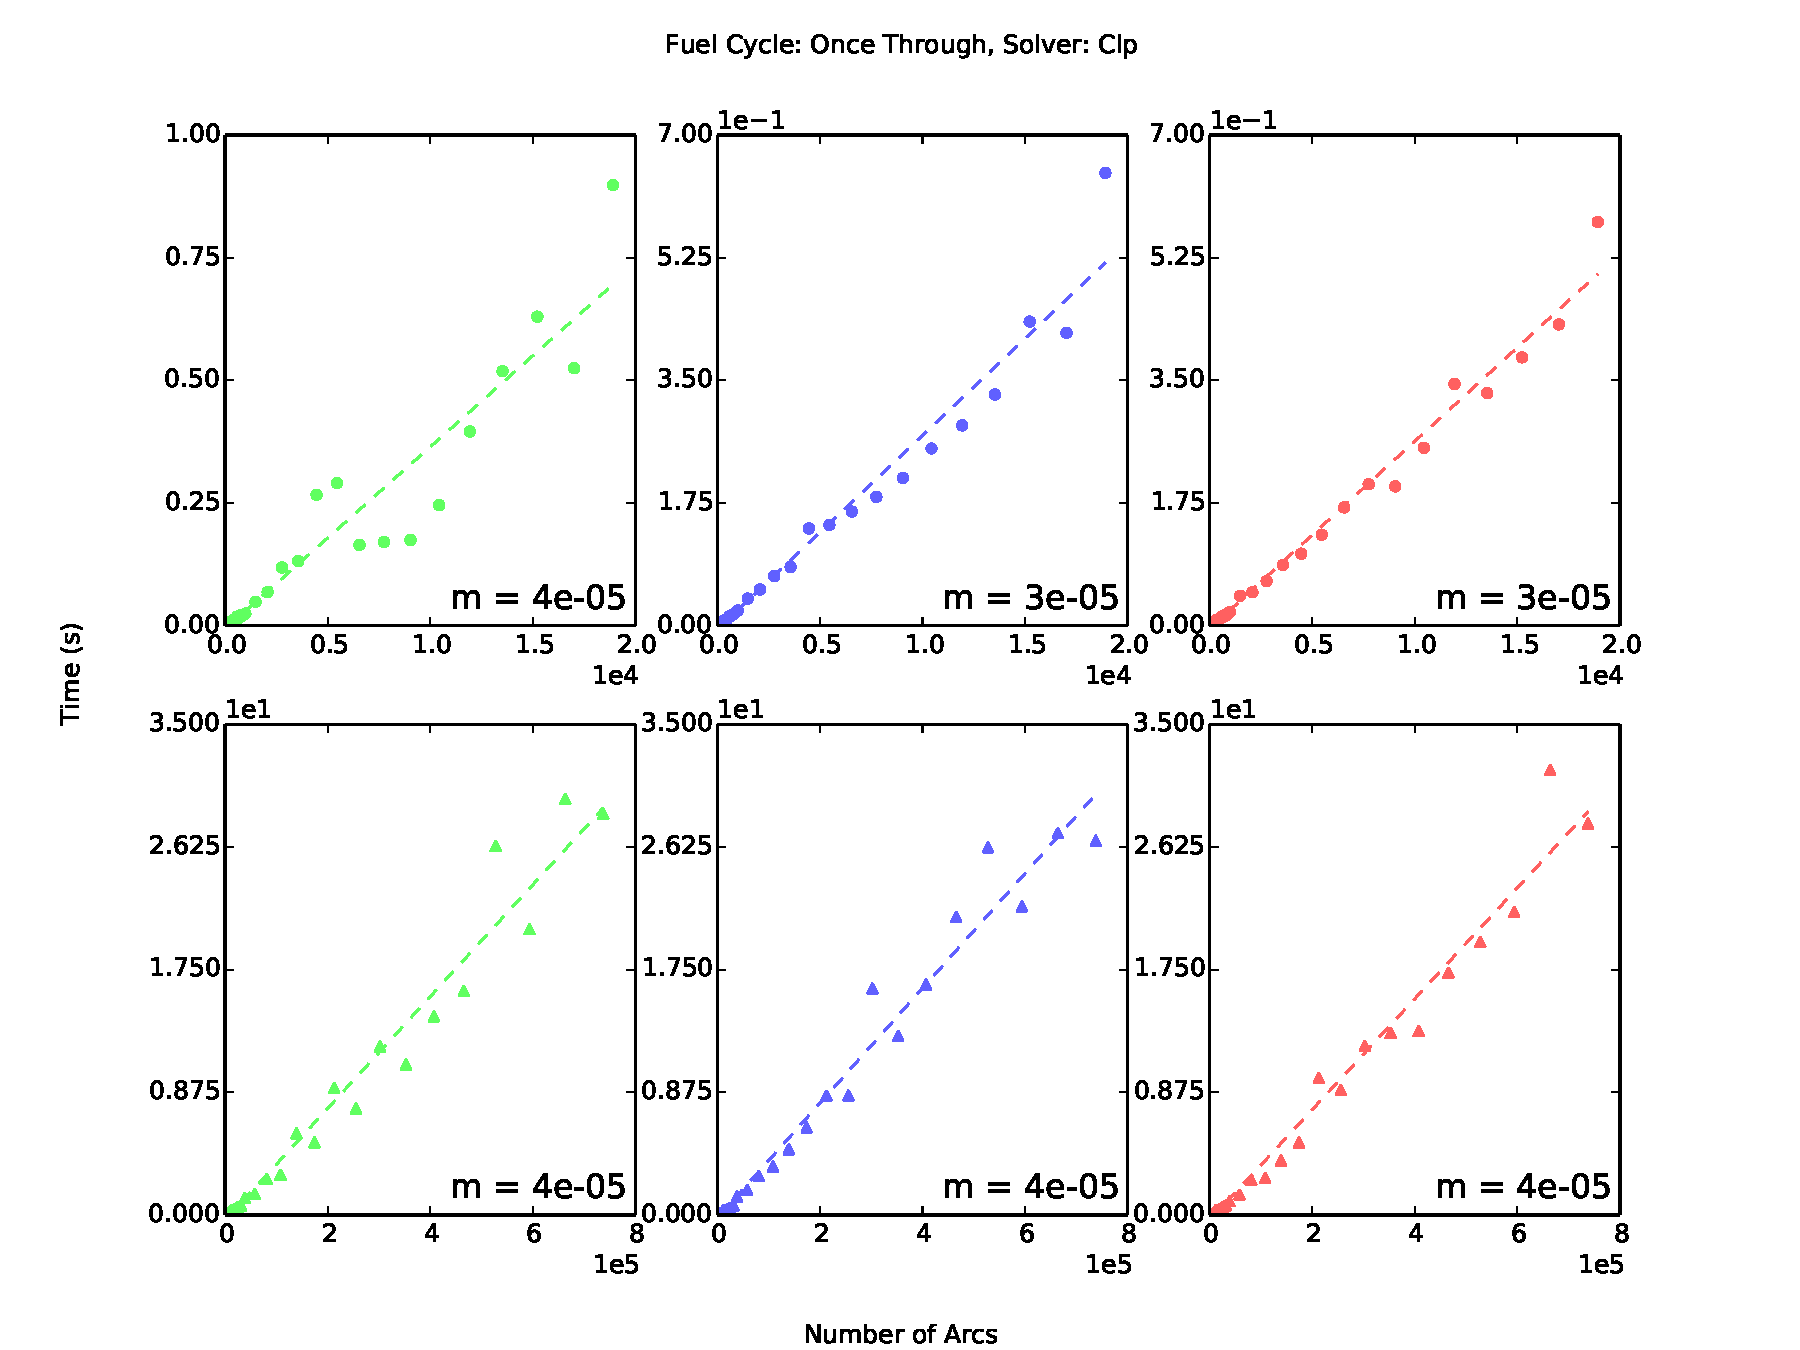
\includegraphics[width=.7\textwidth]{base_front_n_arcs_time_fc0_clp.pdf}
    \caption[]{
      \label{fig:base_front_n_arcs_time_fc0_clp}
      CLP Solver results for the OT fuel cycle as the number of arcs
      increases.
      }
  \end{center}
\end{figure}

\begin{figure}[h!]
  \begin{center}
    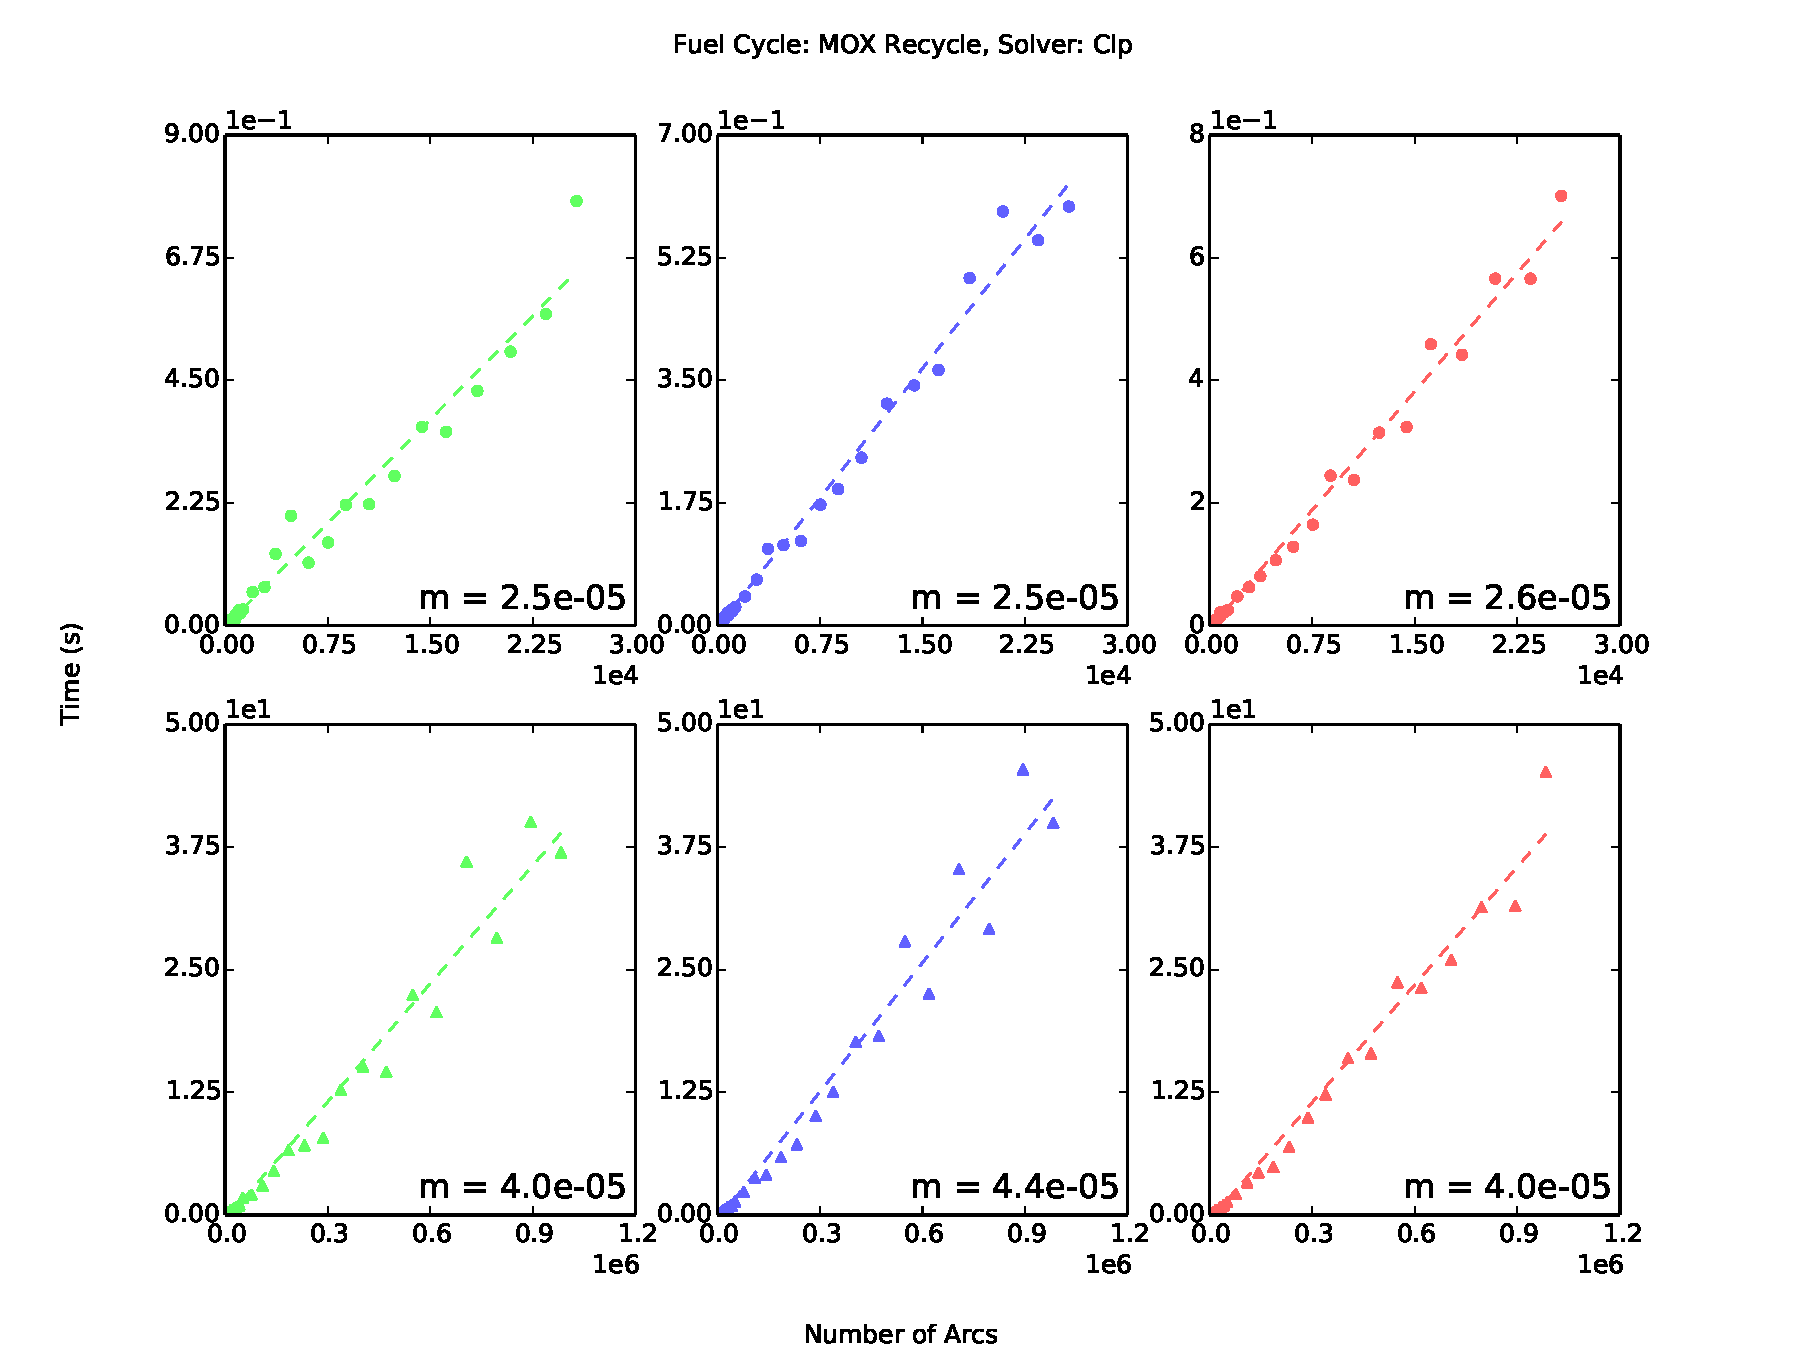
\includegraphics[width=.7\textwidth]{base_front_n_arcs_time_fc1_clp.pdf}
    \caption[]{
      \label{fig:base_front_n_arcs_time_fc1_clp}
      CLP Solver results for the MOX fuel cycle as the number of arcs
      increases.
      }
  \end{center}
\end{figure}

\begin{figure}[h!]
  \begin{center}
    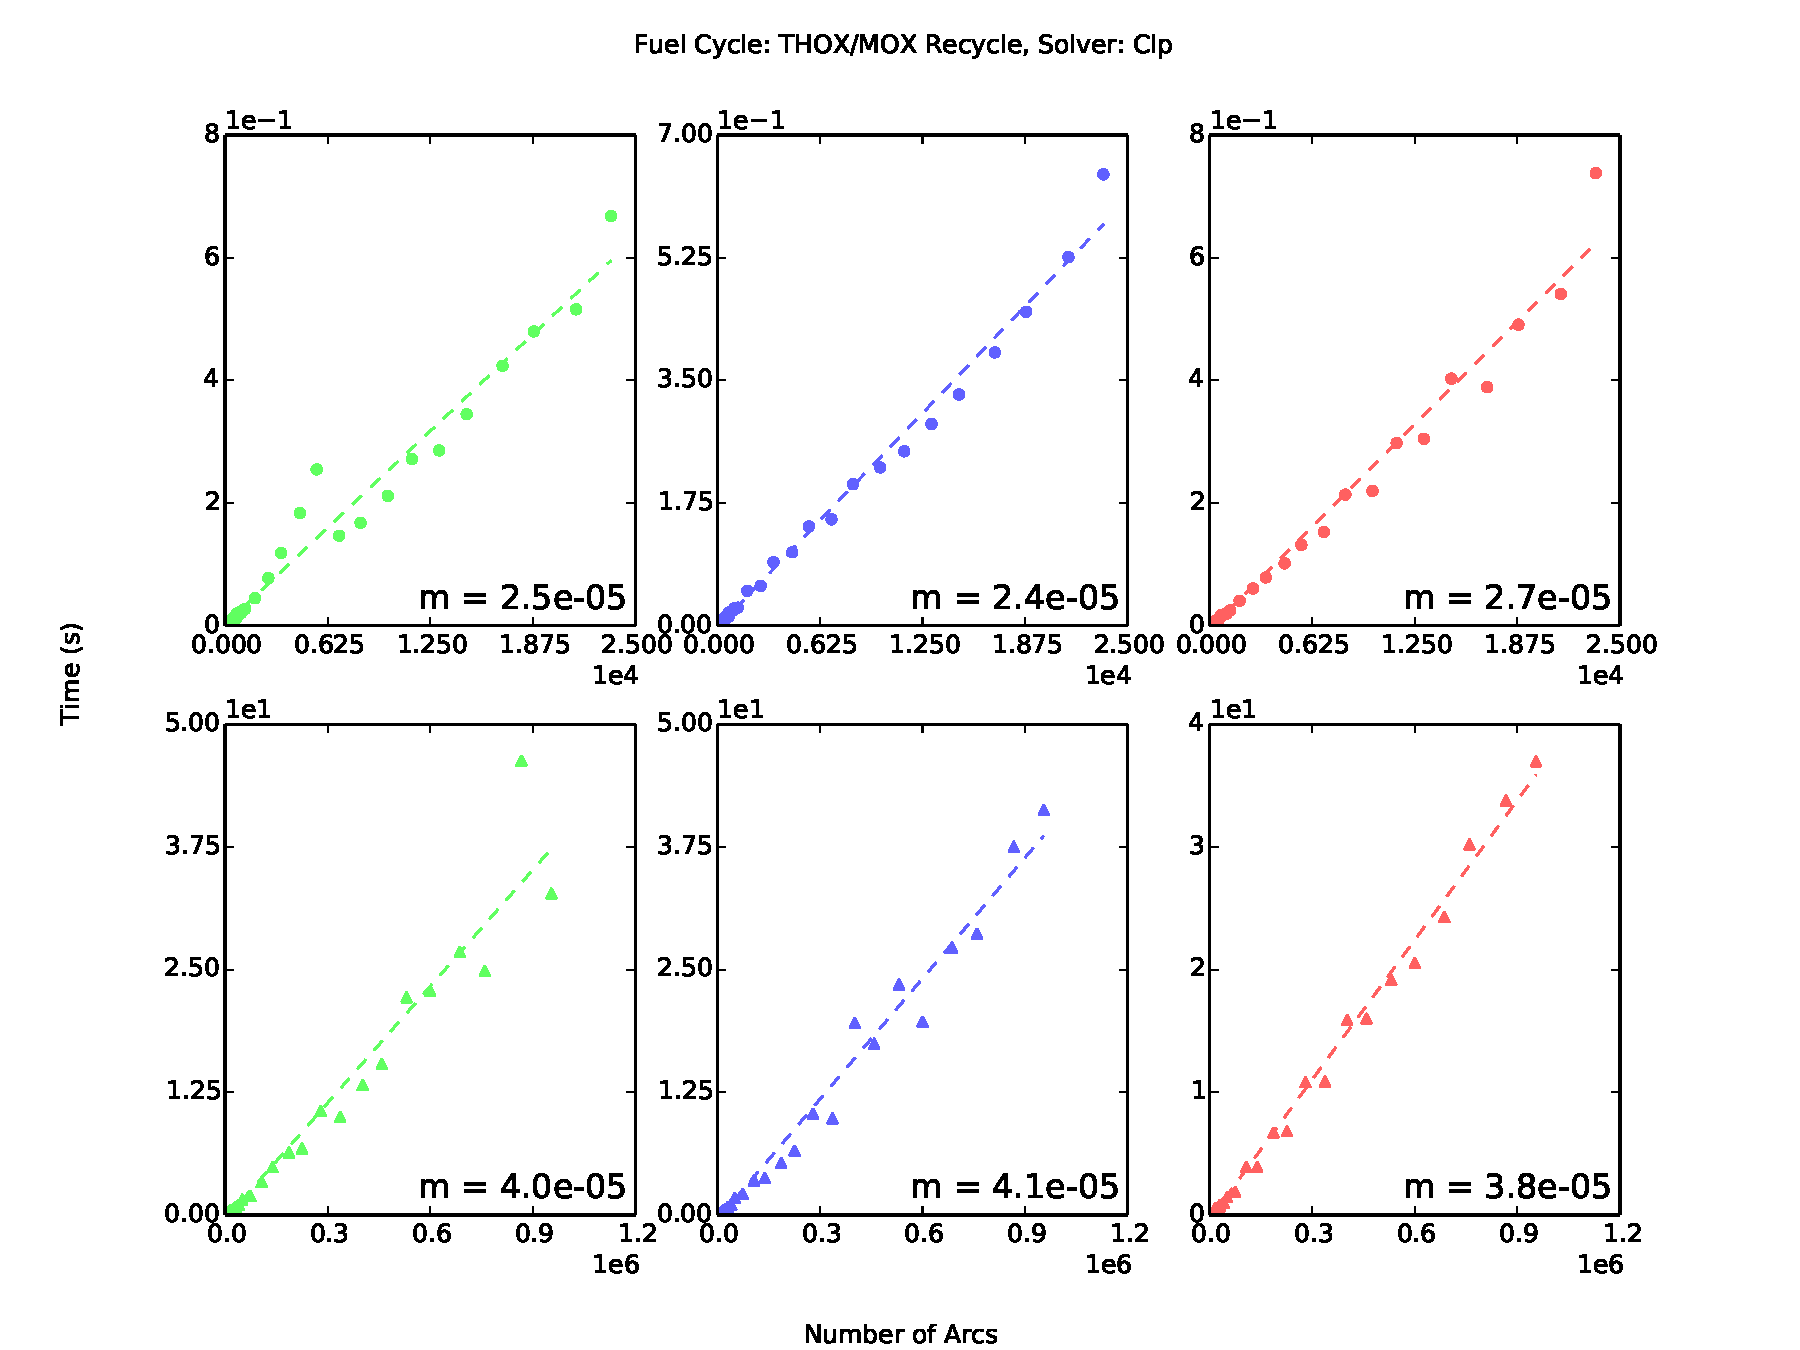
\includegraphics[width=.7\textwidth]{base_front_n_arcs_time_fc2_clp.pdf}
    \caption[]{
      \label{fig:base_front_n_arcs_time_fc2_clp}
      CLP Solver results for the ThOX fuel cycle as the number of arcs
      increases.
      }
  \end{center}
\end{figure}

\paragraph{CBC Solver}

The performance of the CBC solver is much more sporadic than either the CLP or
Greedy solvers. This is to be expected, for MILP optimization problems are
NP-Hard. Cbc was limited to 3 hours for each problem, and a 1\% ratio-gap
convergence criteria was applied. The term \textit{ratio gap} is in reference to
the current known upper and lower bound on the optimal objective value. The
solver reports an optimal solution when the criteria shown in Equation
\ref{eqn:ratio_gap} is true.

\begin{equation}\label{eqn:ratio_gap}
\frac{z_U - z_L}{z_U} \leq 0.01
\end{equation}

In each of the figures below, only instances reaching convergence are displayed
in order to attempt to ascertain any related
trends. \Cref{fig:base_front_n_rxtr_time_fc0_cbc,fig:base_front_n_rxtr_time_fc1_cbc,fig:base_front_n_rxtr_time_fc2_cbc}
show timing results as a function of the number of reactors in the
system. \Cref{fig:base_front_n_arcs_time_fc0_cbc,fig:base_front_n_arcs_time_fc1_cbc,fig:base_front_n_arcs_time_fc2_cbc}
show timing results as a function of the number of arcs in the system. Note that
in each case below, a log-lin graph is used. In each frame, the percentage of
converged instances is provided.

\begin{figure}[h!]
  \begin{center}
    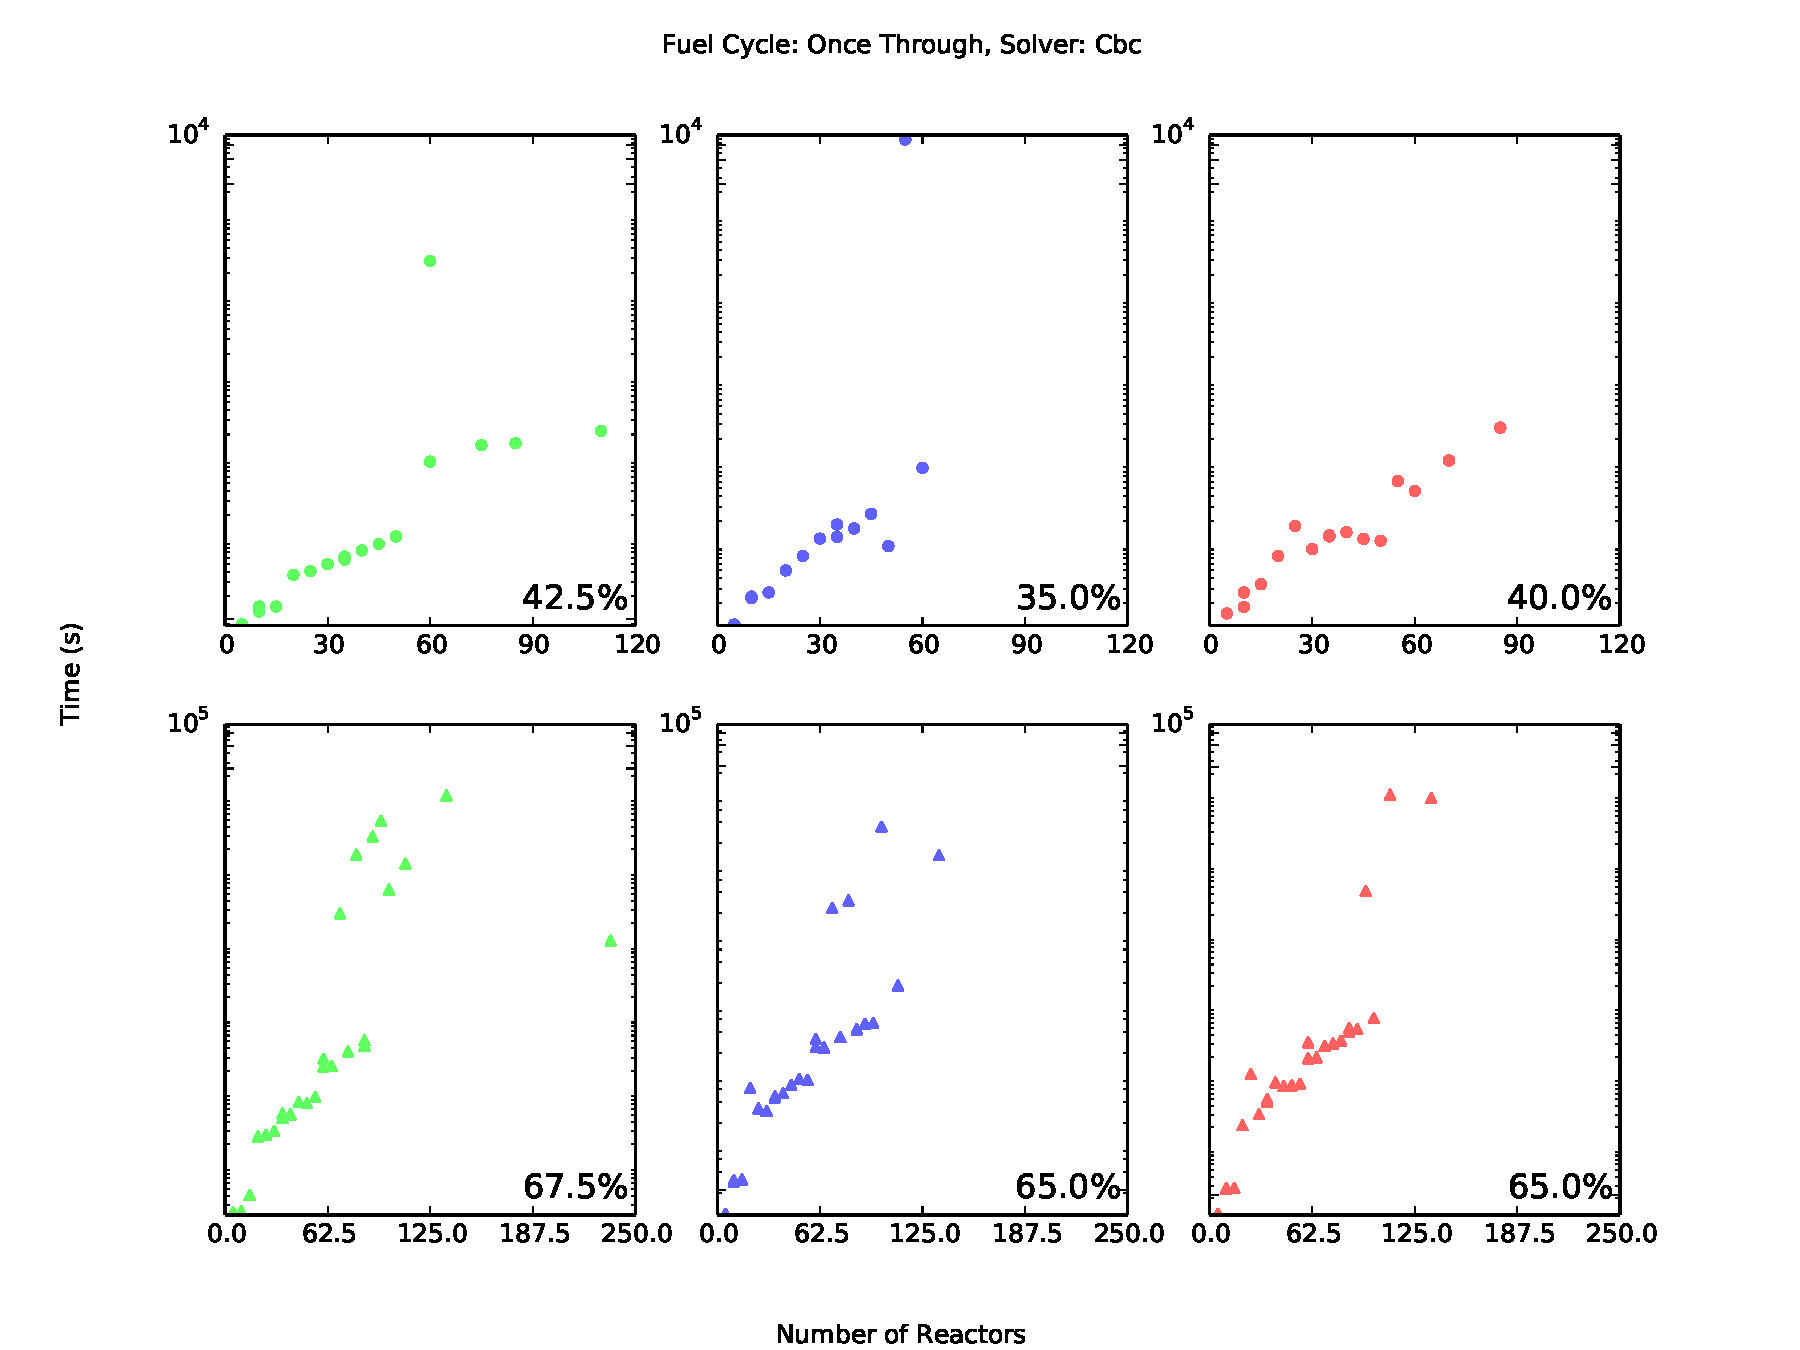
\includegraphics[width=.7\textwidth]{base_front_n_rxtr_time_fc0_cbc.pdf}
    \caption[]{
      \label{fig:base_front_n_rxtr_time_fc0_cbc}
      CBC Solver results for the OT fuel cycle as the number of reactors
      increases.
      }
  \end{center}
\end{figure}

\begin{figure}[h!]
  \begin{center}
    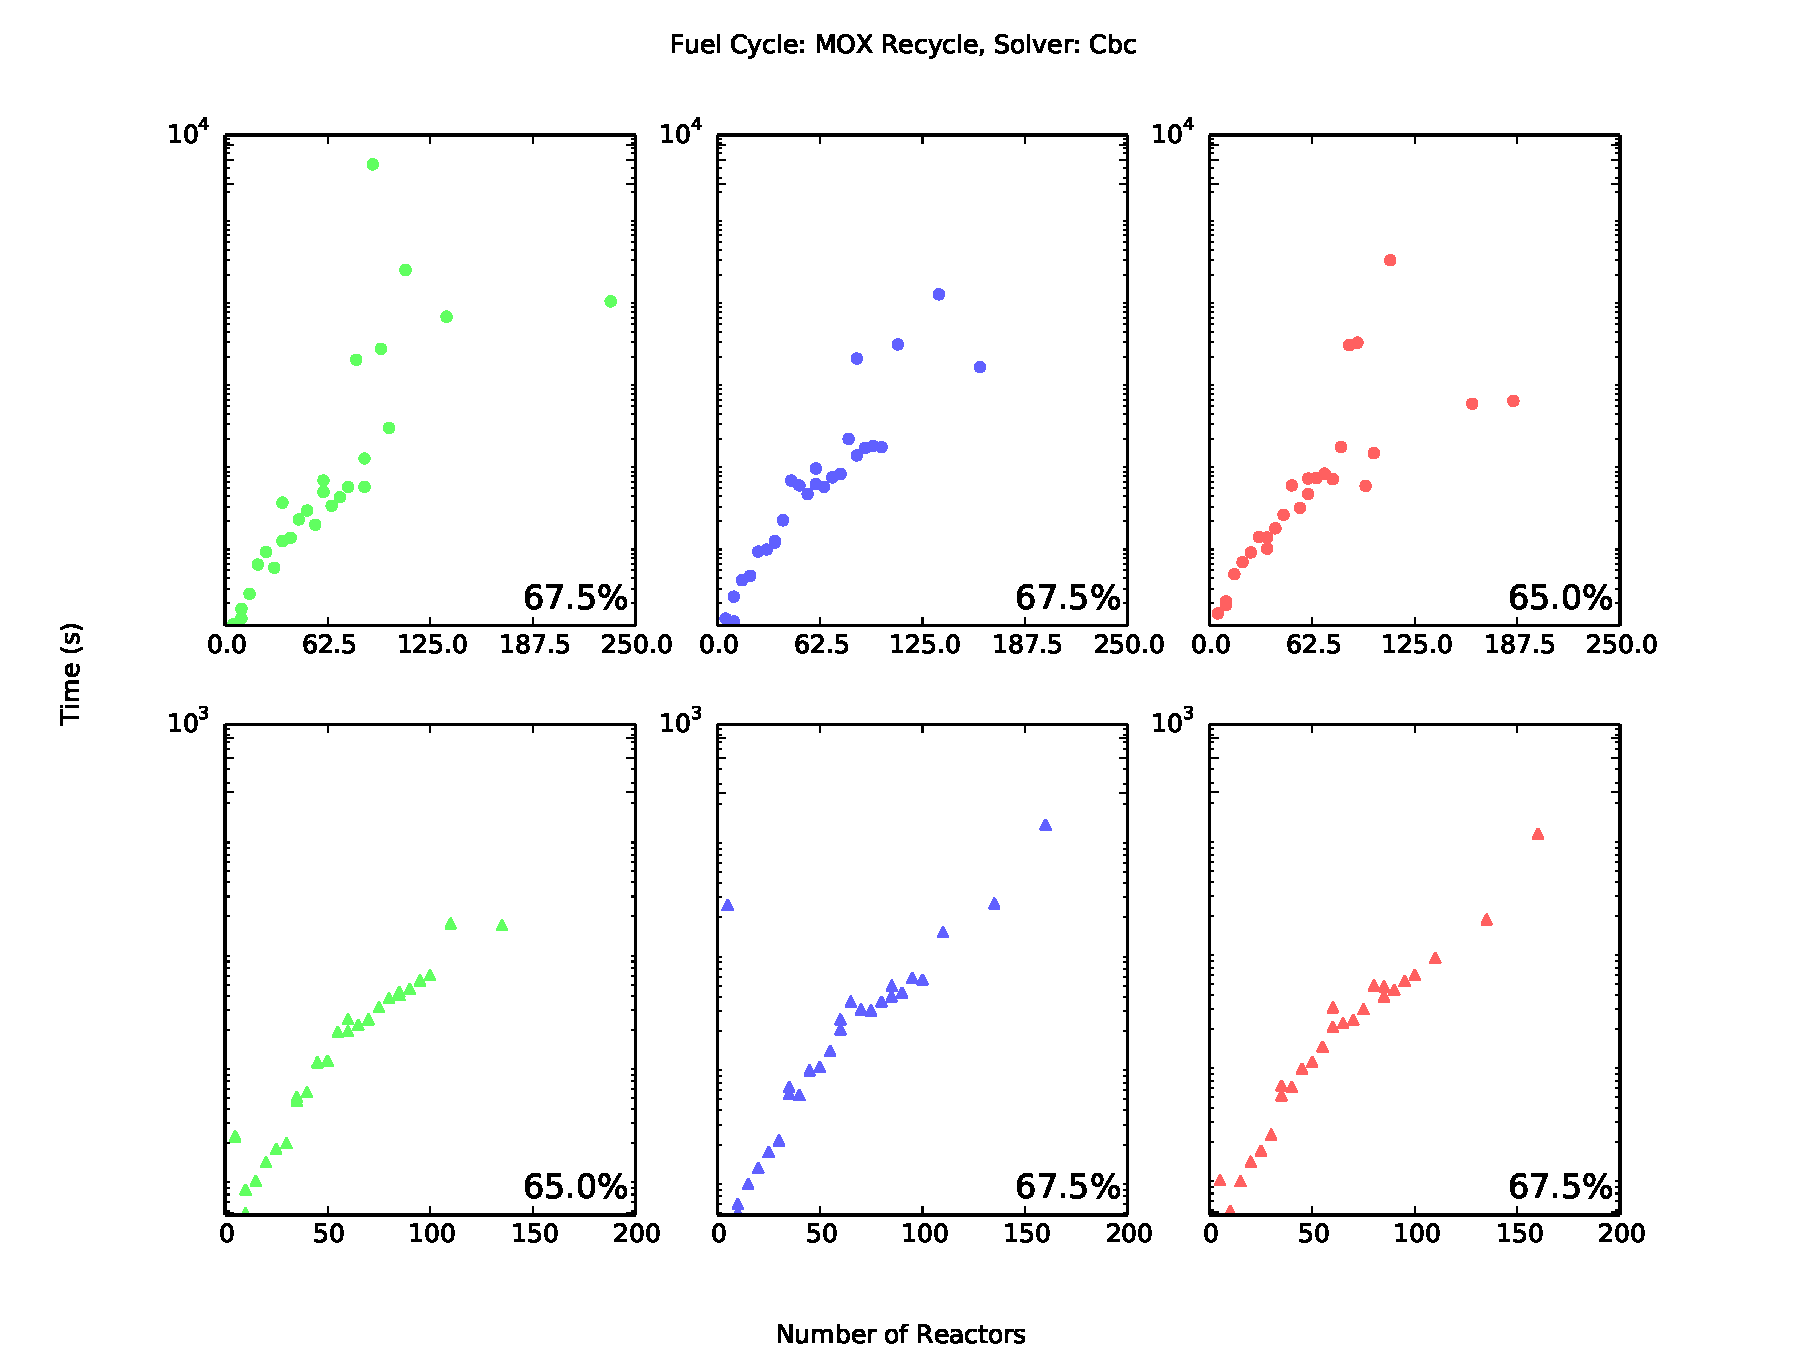
\includegraphics[width=.7\textwidth]{base_front_n_rxtr_time_fc1_cbc.pdf}
    \caption[]{
      \label{fig:base_front_n_rxtr_time_fc1_cbc}
      CBC Solver results for the MOX fuel cycle as the number of reactors
      increases.
      }
  \end{center}
\end{figure}

\begin{figure}[h!]
  \begin{center}
    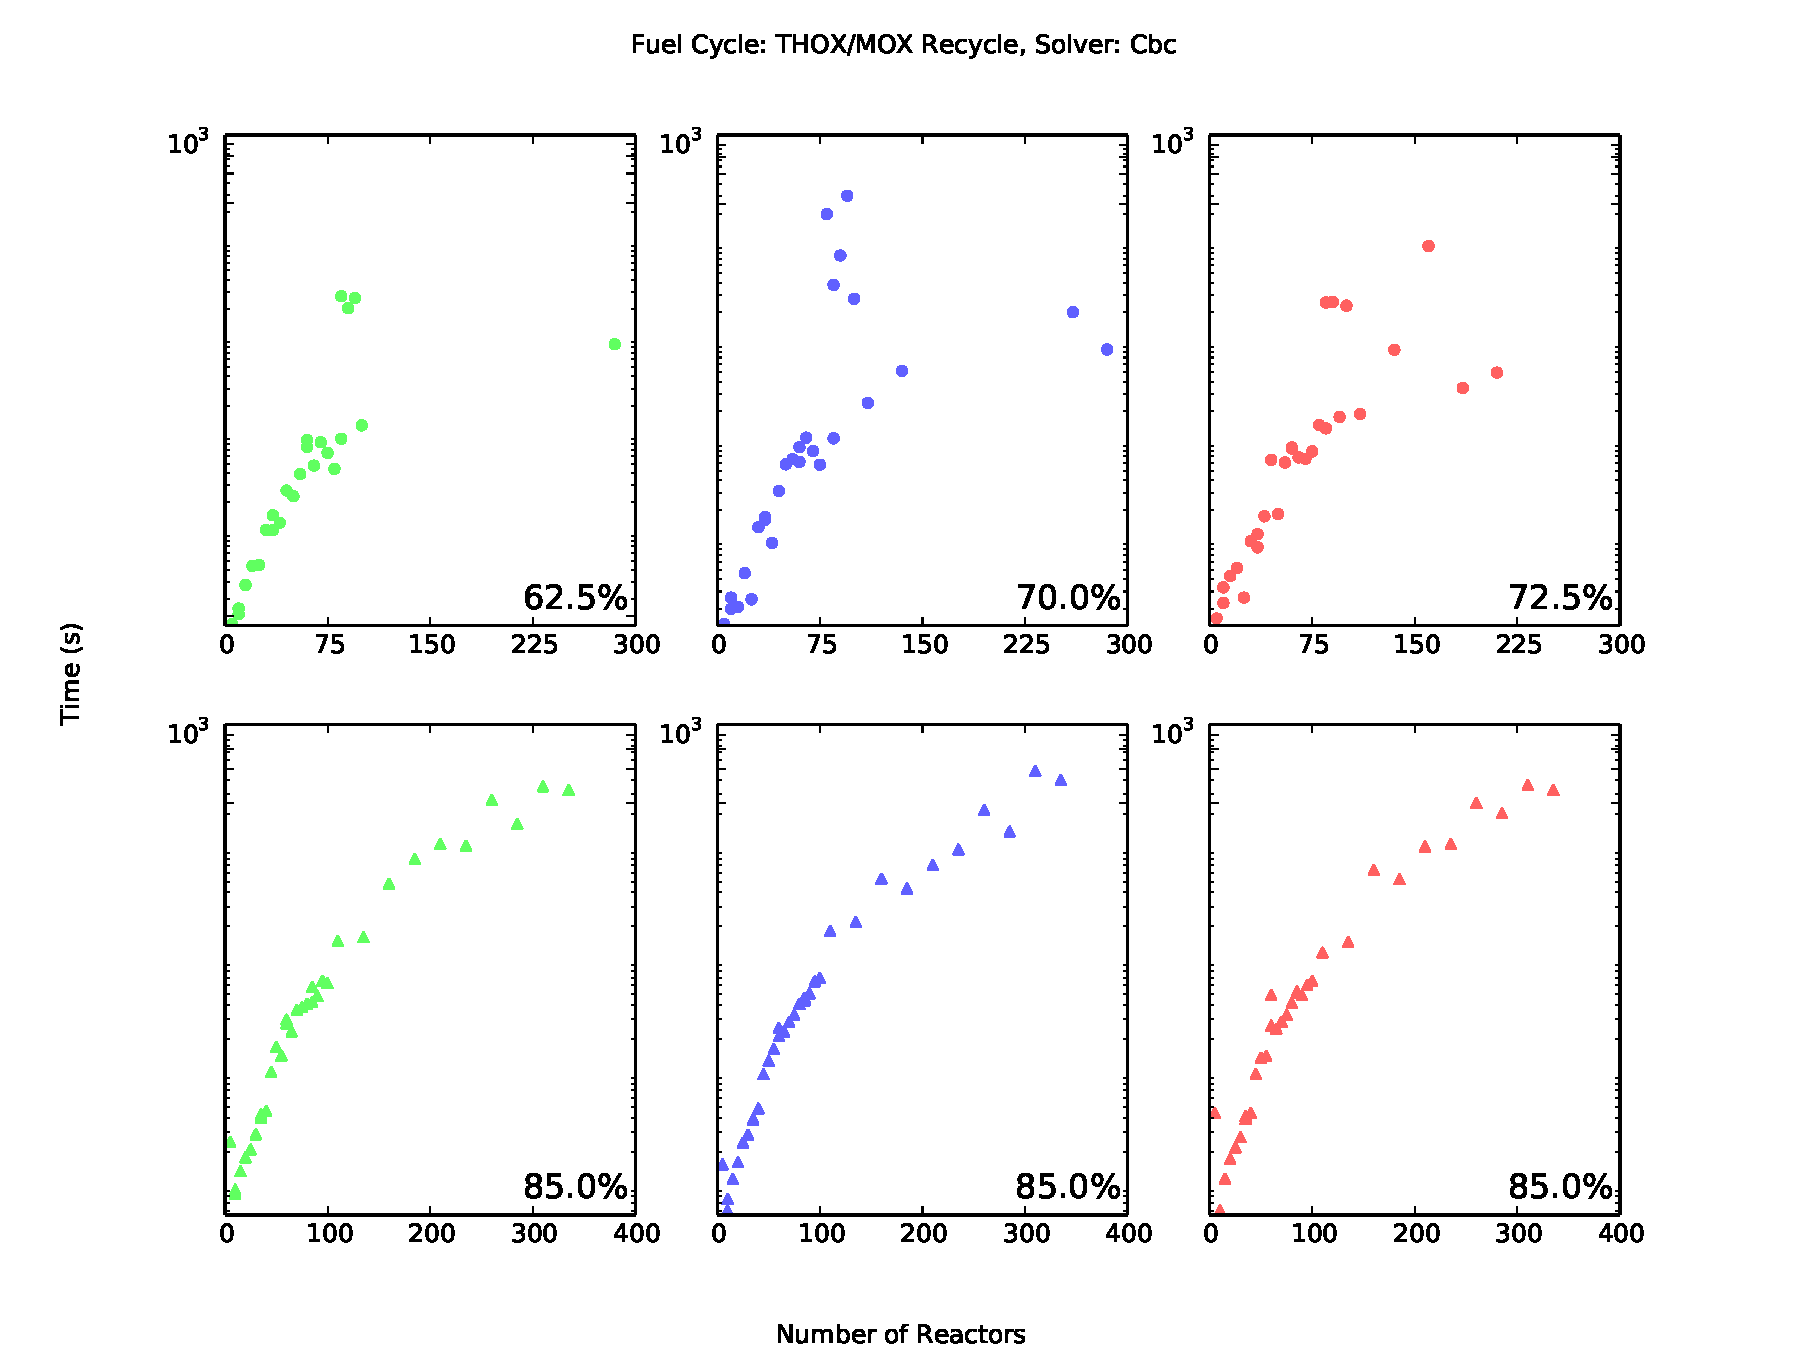
\includegraphics[width=.7\textwidth]{base_front_n_rxtr_time_fc2_cbc.pdf}
    \caption[]{
      \label{fig:base_front_n_rxtr_time_fc2_cbc}
      CBC Solver results for the ThOX fuel cycle as the number of reactors
      increases.
      }
  \end{center}
\end{figure}

\begin{figure}[h!]
  \begin{center}
    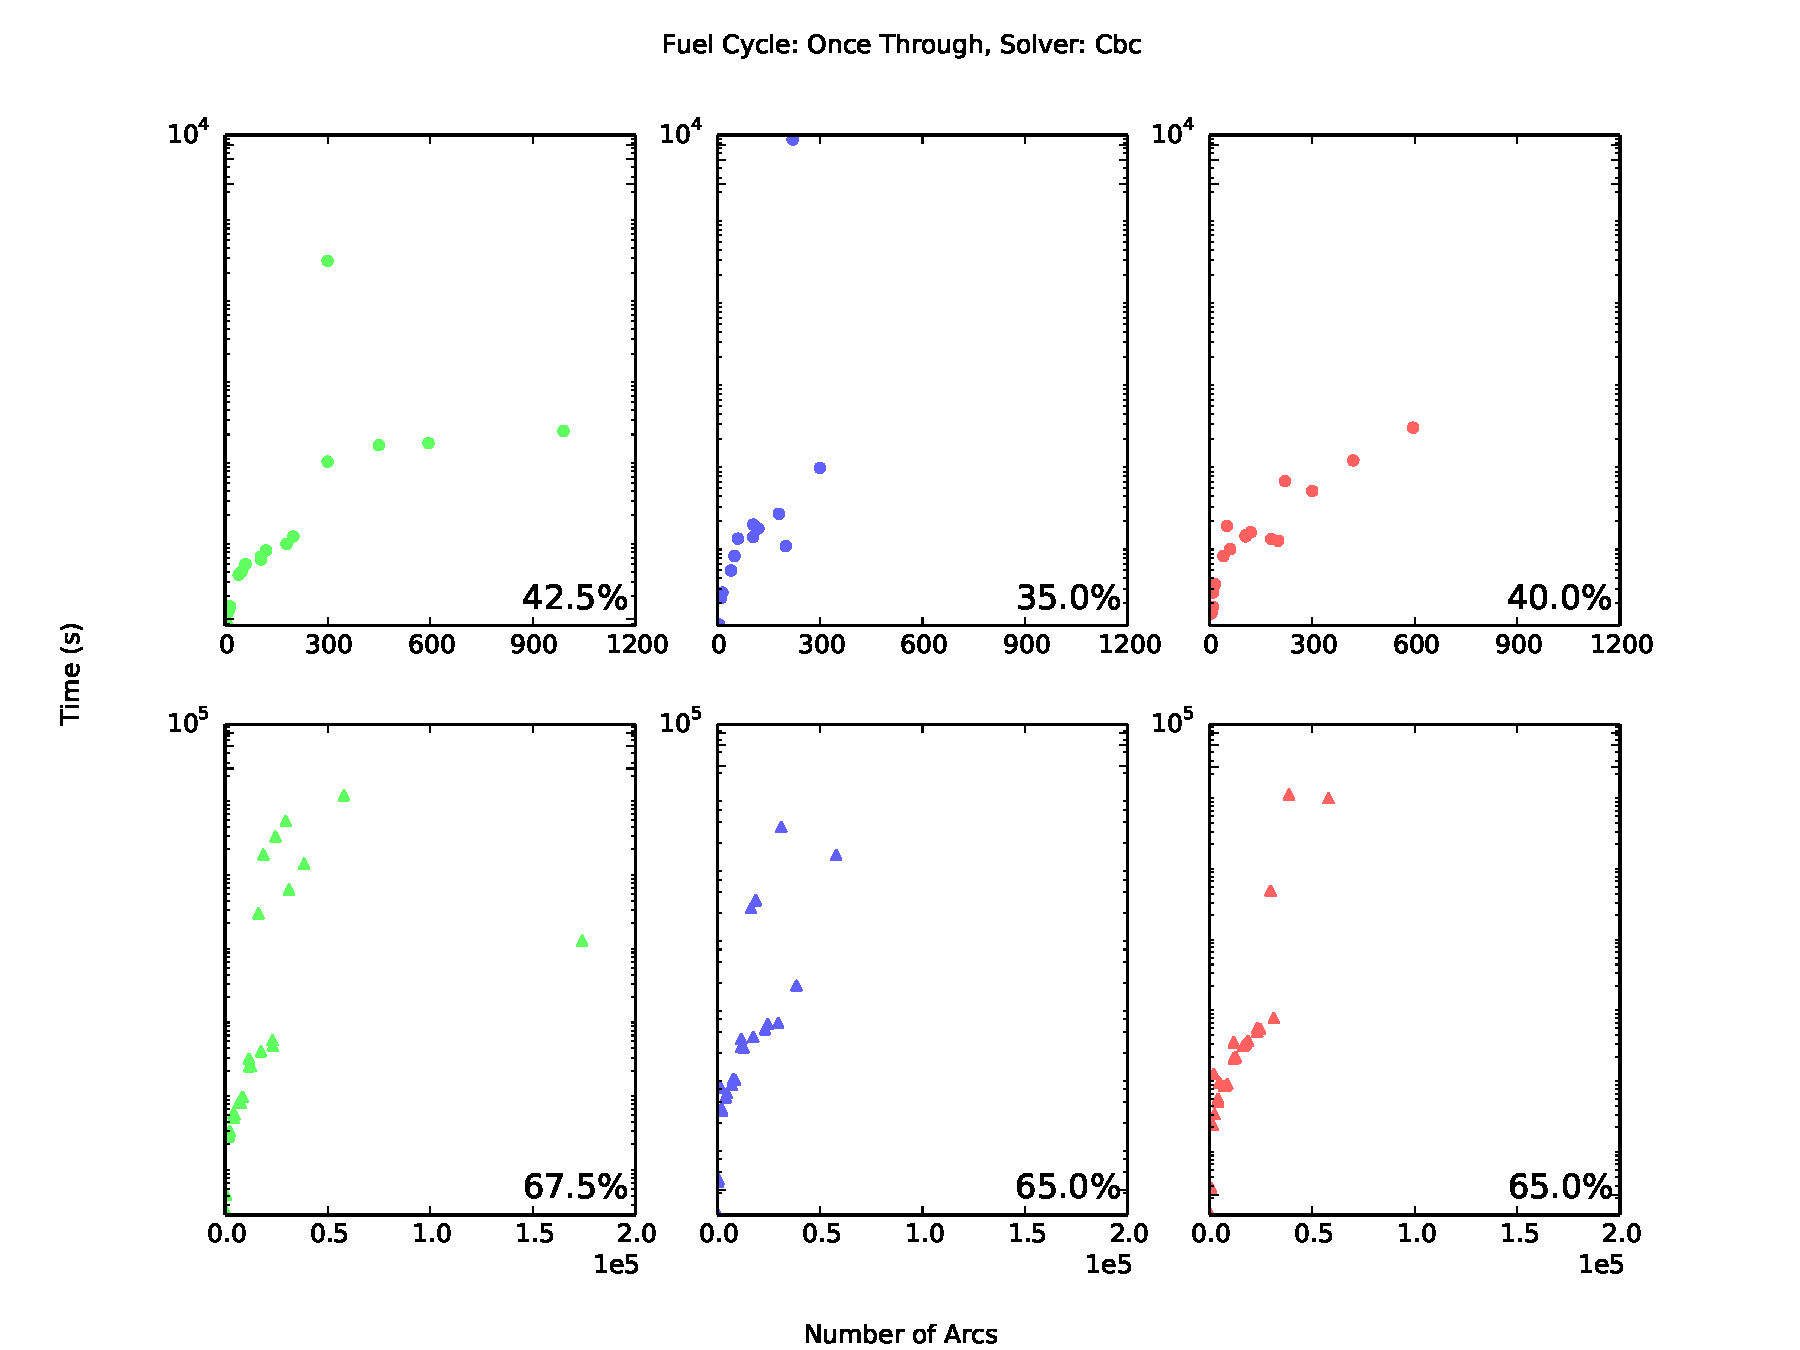
\includegraphics[width=.7\textwidth]{base_front_n_arcs_time_fc0_cbc.pdf}
    \caption[]{
      \label{fig:base_front_n_arcs_time_fc0_cbc}
      CBC Solver results for the OT fuel cycle as the number of arcs
      increases.
      }
  \end{center}
\end{figure}

\begin{figure}[h!]
  \begin{center}
    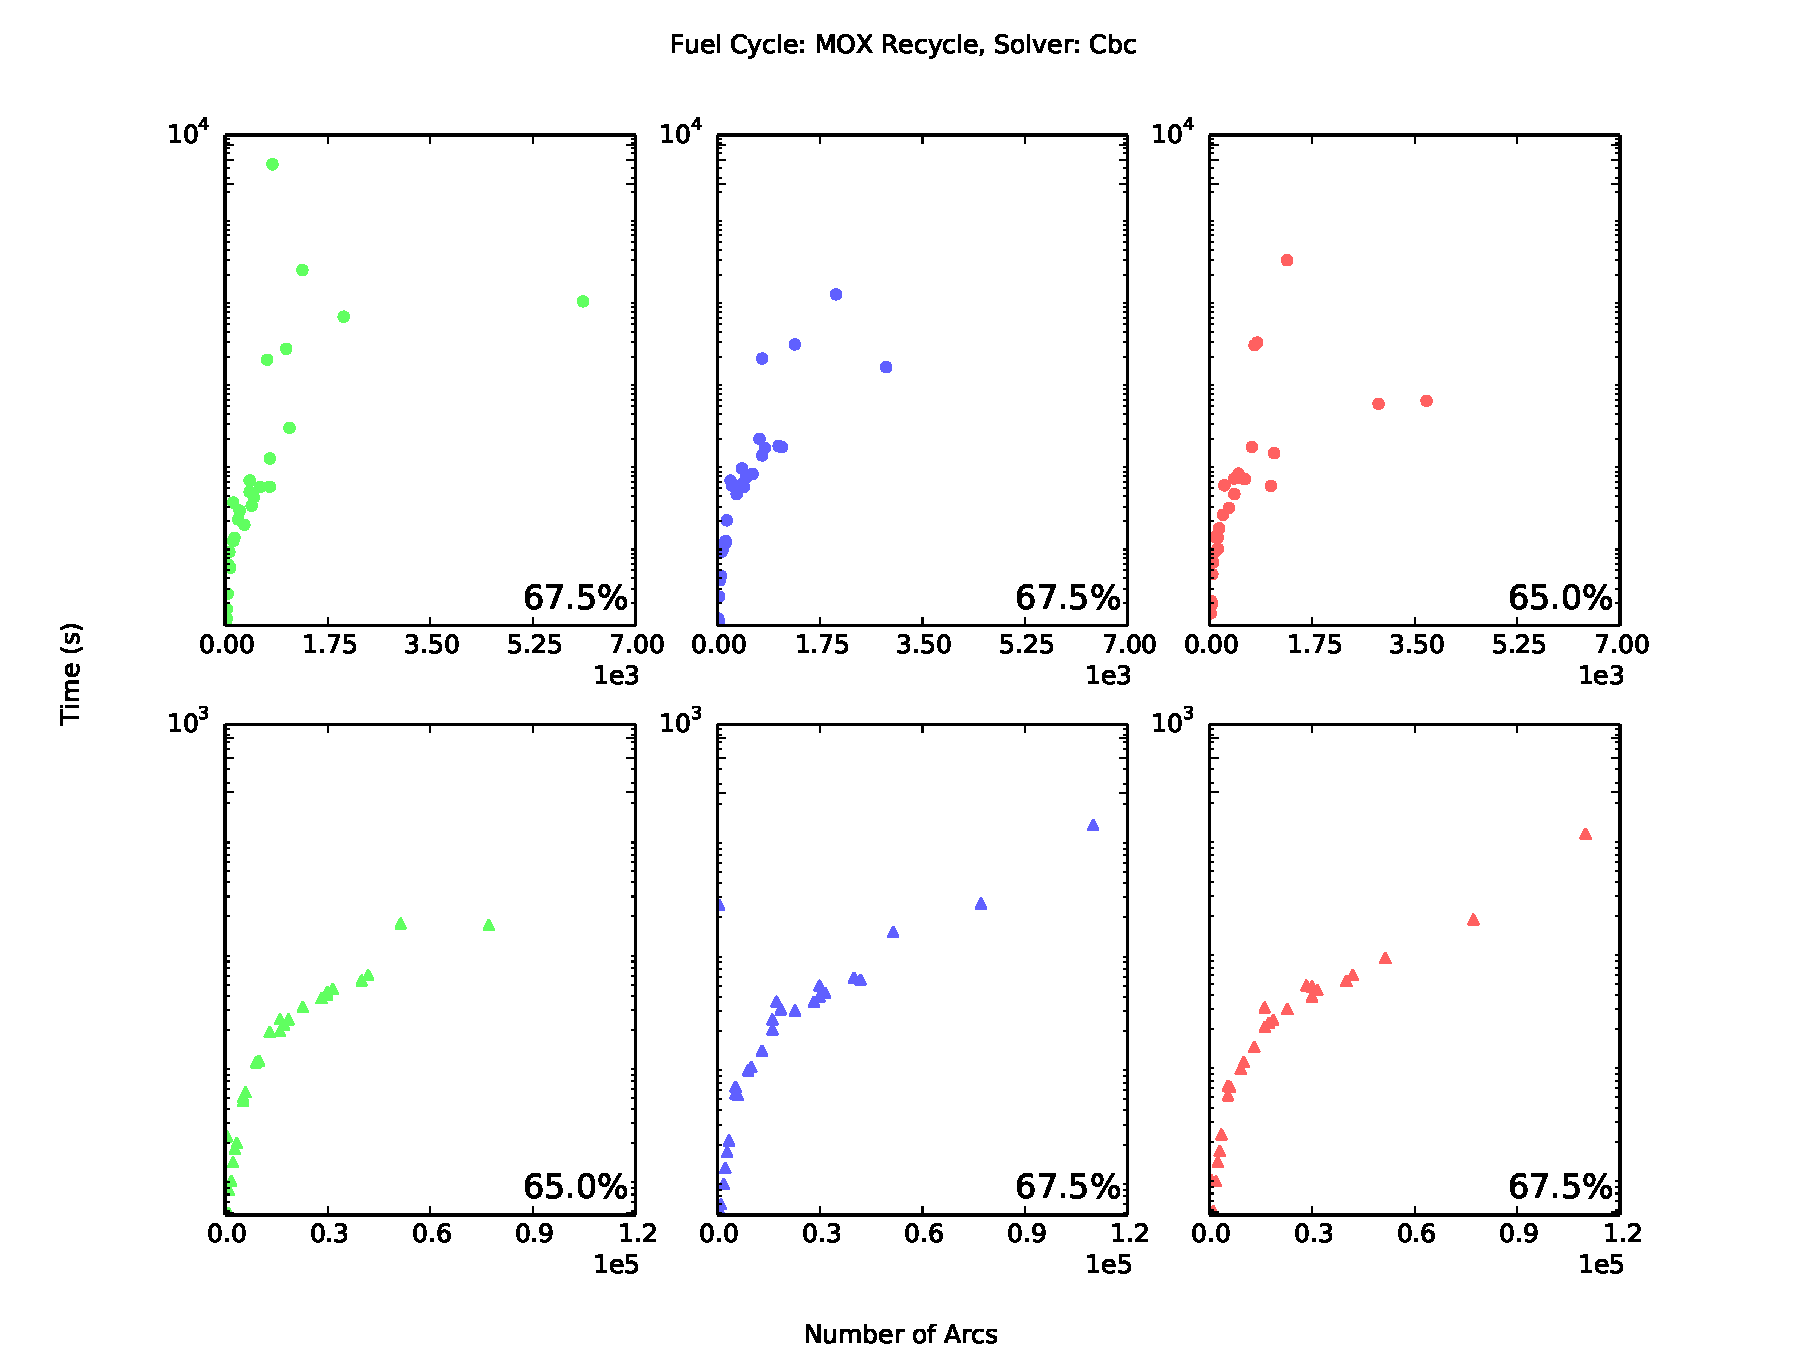
\includegraphics[width=.7\textwidth]{base_front_n_arcs_time_fc1_cbc.pdf}
    \caption[]{
      \label{fig:base_front_n_arcs_time_fc1_cbc}
      CBC Solver results for the MOX fuel cycle as the number of arcs
      increases.
      }
  \end{center}
\end{figure}

\begin{figure}[h!]
  \begin{center}
    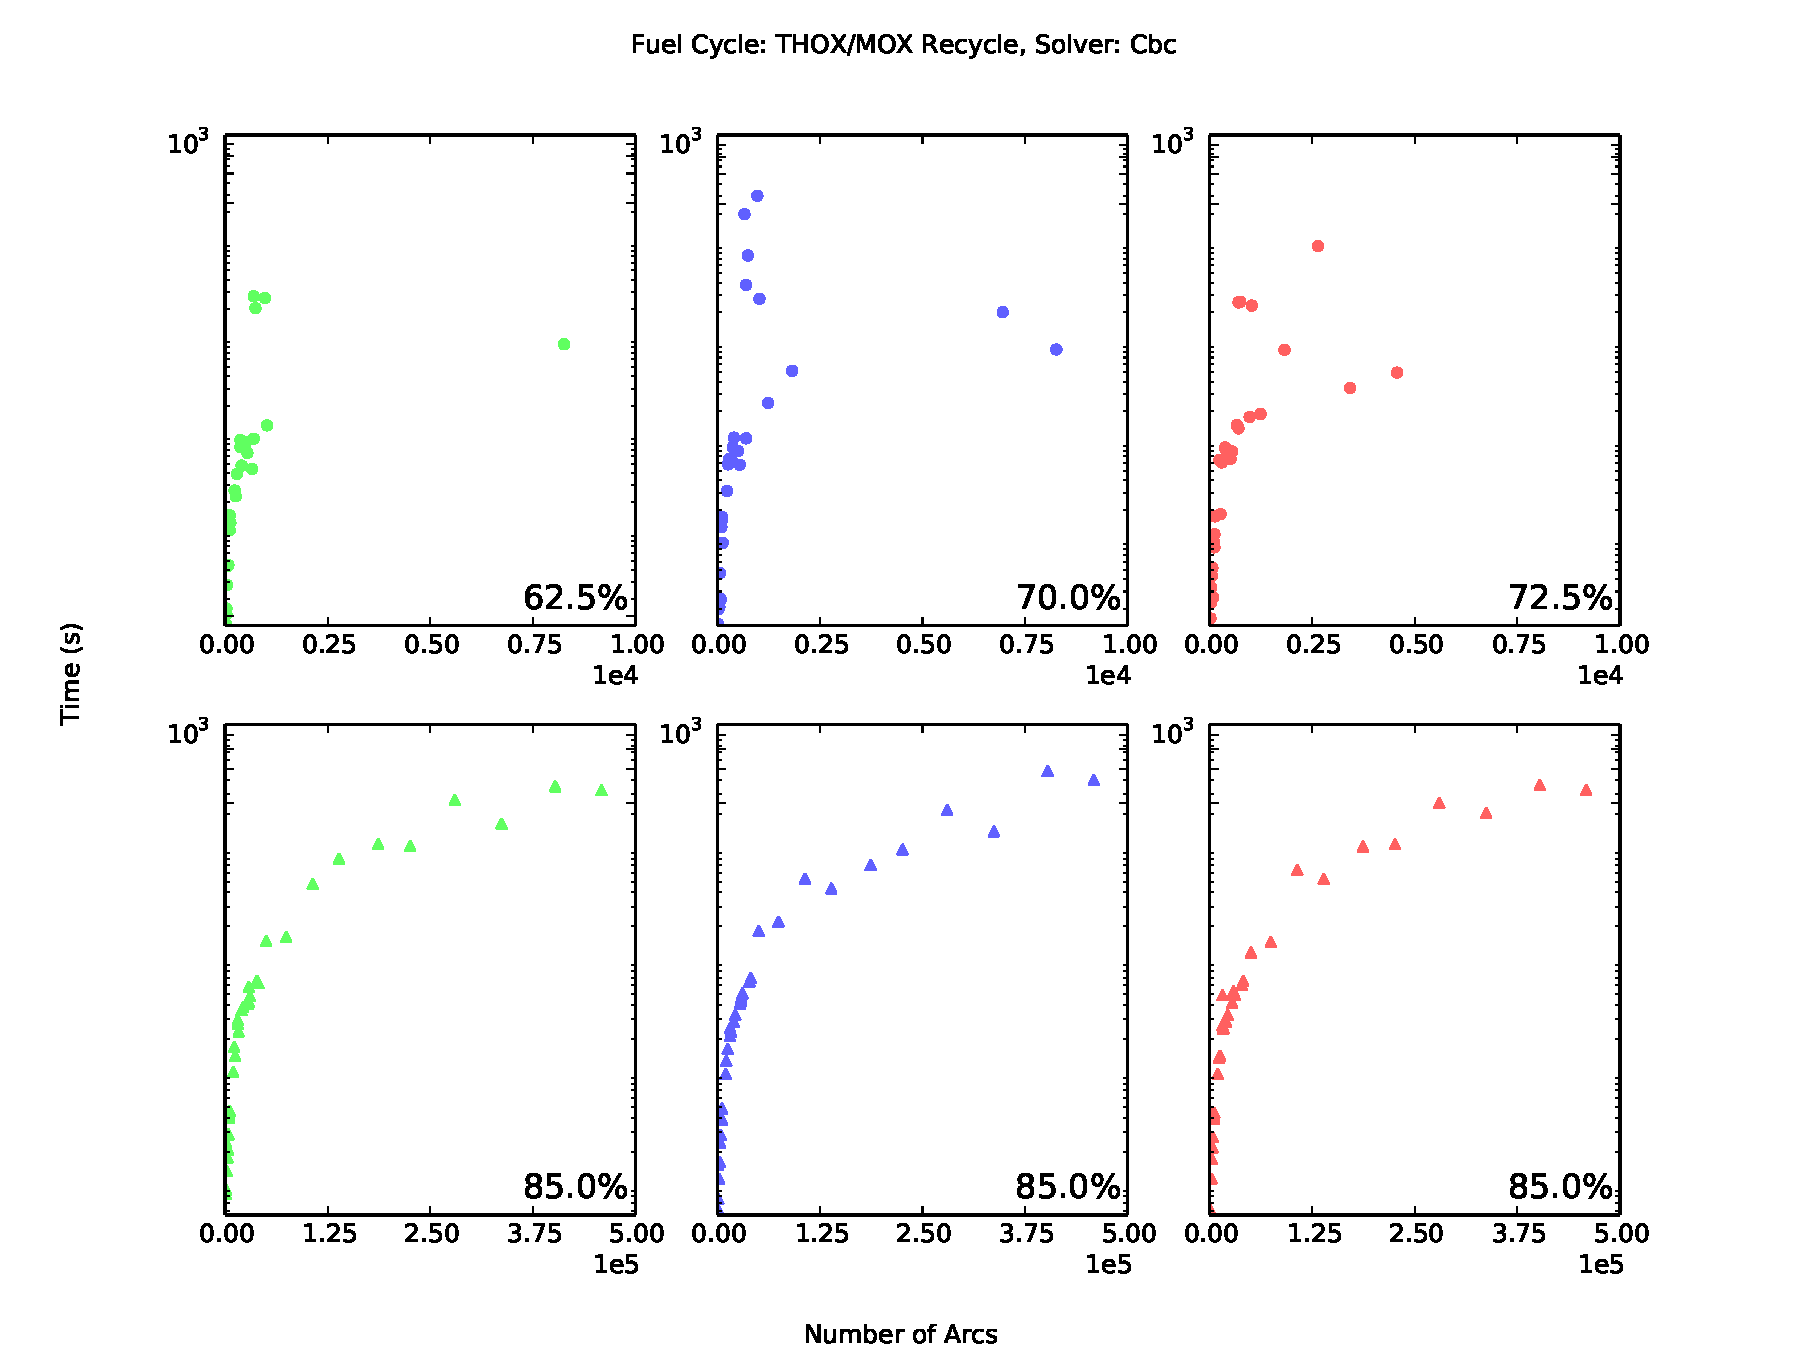
\includegraphics[width=.7\textwidth]{base_front_n_arcs_time_fc2_cbc.pdf}
    \caption[]{
      \label{fig:base_front_n_arcs_time_fc2_cbc}
      CBC Solver results for the ThOX fuel cycle as the number of arcs
      increases.
      }
  \end{center}
\end{figure}

Immediately obvious, and slightly counter intuitive, is that the population of
converged instances is larger for assembly-based exchanges rather than
batch-based exchanges, even though the number of variables in the problem is
much lower for batch-based exchanges. Additionally, the CBC solver converged in
many fewer instances for low reactor fidelity in the OT fuel cycle than either
MOX or ThOX cycles. Low-fidelity once-through cases have the least amount of
``choice'' in the system. There is a single commodity, consumer type, and
supplier type. Regardless of fuel cycle, reactor fidelity, or objective
coefficient strategy, the Cbc solver experiences exponential scaling with
problem size.

\subsubsection{Solution Comparison}\label{sec:res:scale:front:soln}

Solutions between any two solvers can be compared either in the formulation
layer or in the exchange layer. Comparison in the formulation layer is achieved
by comparing objective function values (Equation \ref{eqn:obj_flow}), whereas
comparison in the exchange layer is achieved by comparing a measure the flows
and preferences for a given solution (Equation \ref{eqn:sim_flow}). The
objective function includes the costs and flows on false arcs which inflates the
objective function value. While the false arcs are necessary for guaranteeing a
feasible solution, their resulting flows are not taken into account when the DRE
back-translates from the formulation to the exchange layer. Accordingly, a
measure of the preference and flow, as shown in Equation \ref{eqn:sim_flow}, is
used to compare results between solvers.

Comparisons are made between the Greedy solver and the CBC solver when the CBC
solver, provided the CBC solver converged. Because solutions increase in
magnitude with increasing problem size, a relative comparison is made, as shown
in Equation \ref{eqn:sim_flow_compare}. The resulting features are similar
across fuel cycles. Accordingly, an example for the MOX fuel cycle is shown in
Figure \ref{fig:compare_cbc_greedy_pref_flow_front_n_rxtr__fc1_}.

\begin{equation}\label{eqn:sim_flow_compare}
\frac{z^*_{\text{sim}} - z_{\text{sim}, \text{Greedy}}}
     {z^*_{\text{sim}}} 
\end{equation}

\begin{figure}[h!]
  \begin{center}
    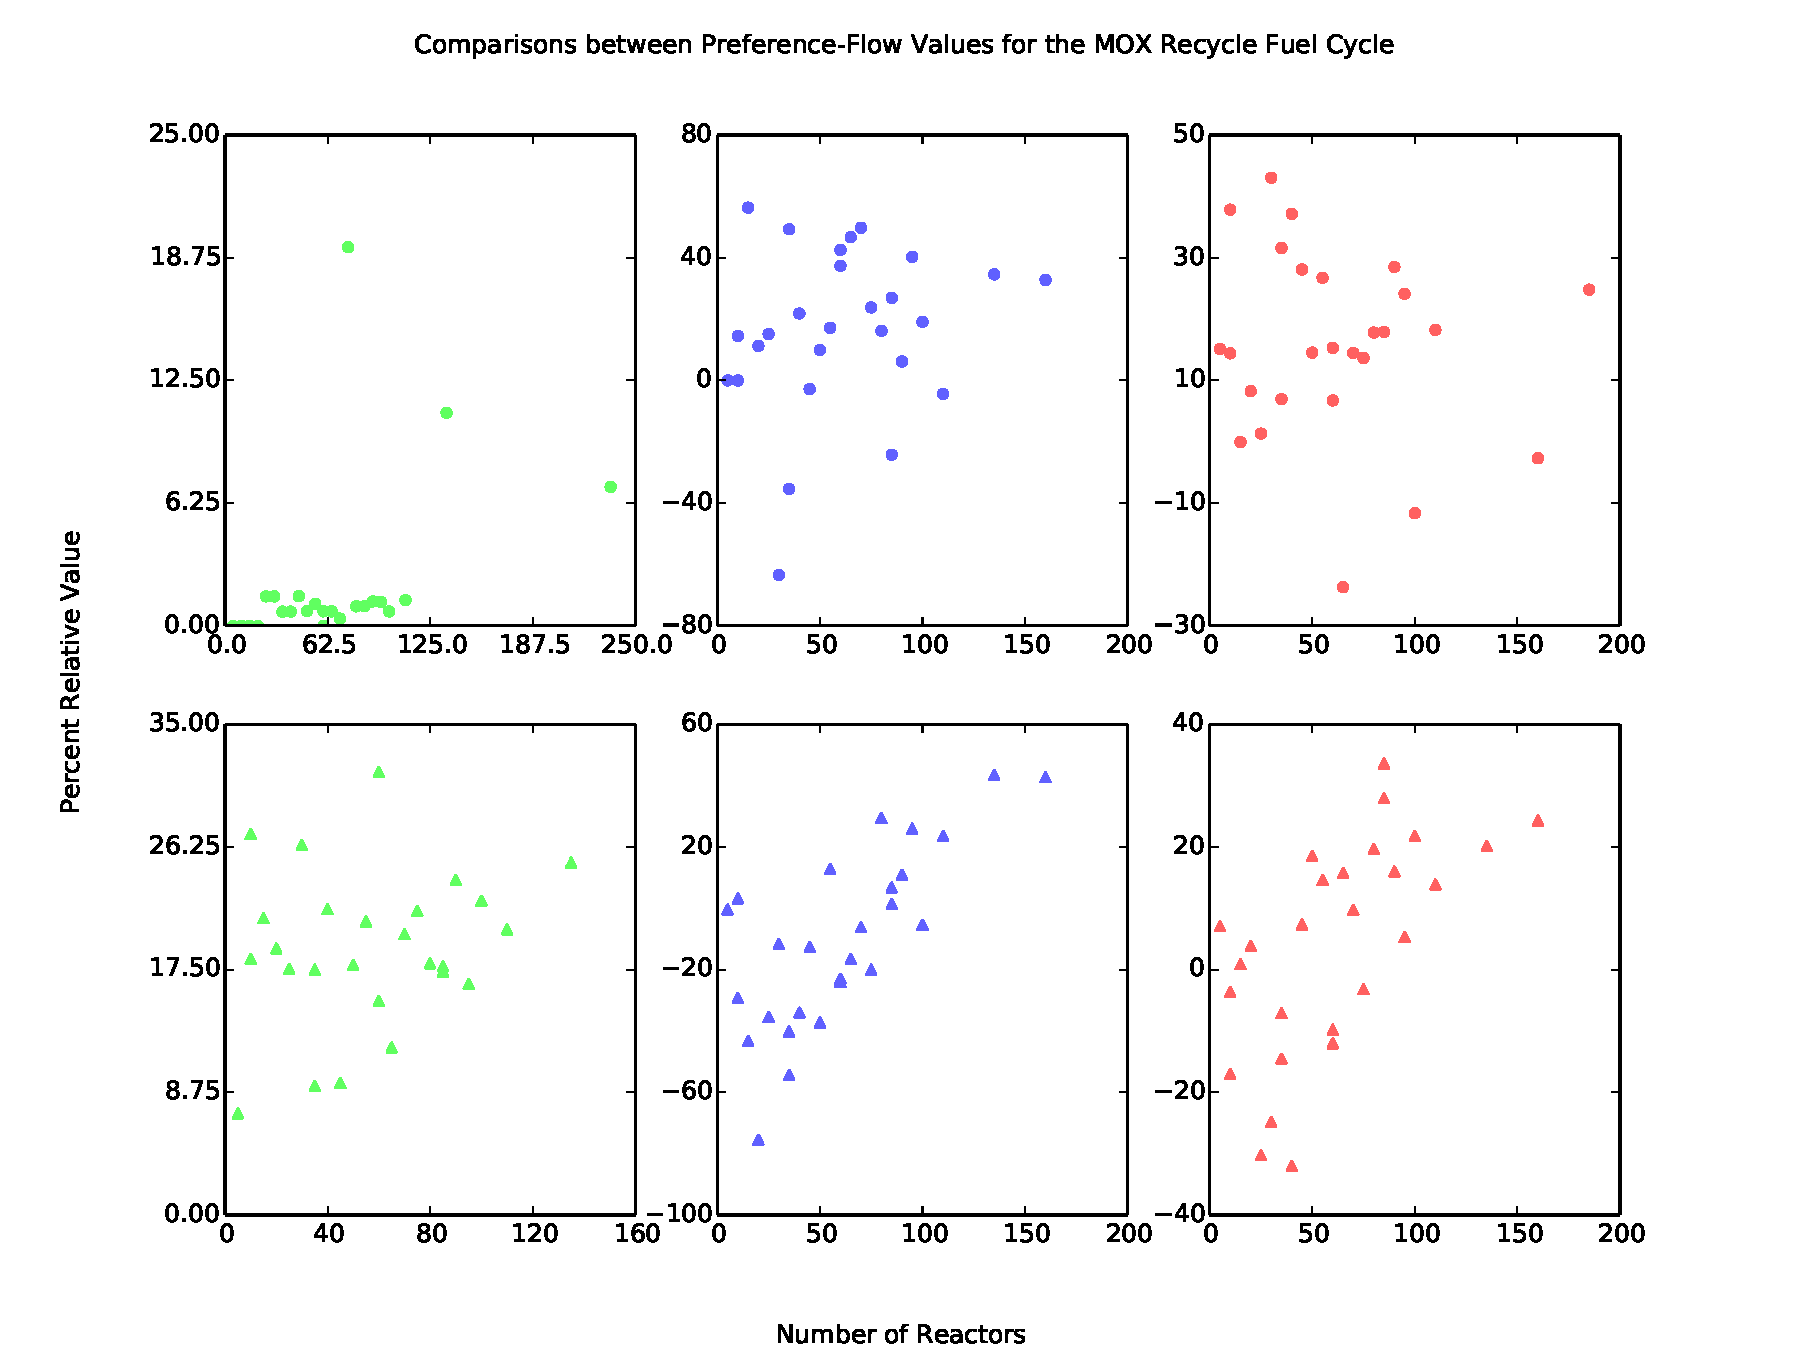
\includegraphics[width=.7\textwidth]{compare_cbc_greedy_pref_flow_front_n_rxtr__fc1_.pdf}
    \caption[]{
      \label{fig:compare_cbc_greedy_pref_flow_front_n_rxtr__fc1_}
      Comparisons between relative simulation metrics between the CBC solver and
      the Greedy solver for MOX fuel cycles. Only converged CBC
      solutions are compared.  }
  \end{center}
\end{figure}

Comparing the results in which there are no location-based preferences (green),
there is a clear correlation between the number of variables and the relative
benefit of using CBC. Thus, the Greedy heuristic performs better when the number
of possible assignments is small. As more variety is included in objective
coefficient values via location assignment, the spread of possible values
increases. In other words, the objective function projection on the feasible
space gains more features.

Two features of interest arise when comparing the cases in which there is a
coarse location preference (blue) and a fine location preference (red). First,
some values are negative, implying that the Greedy solver provides a better
preference-space solution than the CBC solver. Importantly, this is true only in
preference space; the CBC always performs better in cost space, by
definition. The Greedy solver is allowed to provide better answers in preference
space for two reasons: the problem is highly constrained, and false arcs have an
arbitrarily high unit cost. CBC converges when the criteria in
\ref{eqn:ratio_gap} is met. When a problem is highly constrained, many false
arcs will be activated, contributing a large amount to the objective
function. If the choice between two possible flows is sufficiently small, i.e.,
small relative to $z^*$, then either solution may be returned upon convergence
depending on the branch-and-bound search path. Thus, good solutions in
preference-space are somewhat lost in the ``noise'' of cost-space.

This effect is reduced when the objective choice in cost-space increase, as
shown in case of fine location preference. In short, the objective function has
a more pronounced shape in cost-space, reducing the heuristic quality and
increasing the quality of the CBC solution. Interestingly, as can be seen in the
lower part of Figure \ref{fig:compare_cbc_greedy_pref_flow_front_n_rxtr__fc1_},
as the number of variables increases (and the quantity associated with each
variable decreases), CBC simulation values decreases in quality with respect to
Greedy solutions. Effectively, more false-arc quantity can be packed into the
solution because there is finer-grained choice for assembly requests than for
batch requests.

The Greedy solver can provide quite good preference-space results relative to
the CBC solver when an exchange is highly constrained \textit{and} when the cost
coefficient assigned to false arcs is relatively large. This effect can be
observed by adjusting the false-arc cost coefficient, e.g., as shown in Equation
\ref{eqn:small_false_cost}. Two exchanges for which the Greedy solver performed
better in preference-space were chosen to demonstrate the effect. The results
are shown in Table \ref{tbl:false_arcs}. Note that it every case, $z$ is smaller
for the Greedy solver than CBC; however, $z_\text{sim}$ for the Greedy solver is
larger than the same value with a large CBC false-arc cost and smaller than
values related to small CBC false-arc costs.

\begin{equation}\label{eqn:small_false_cost}
c_\text{false} = \frac{1}{p_\text{max}} + 1
\end{equation}

\begin{table}[h!]
\centering
\caption{Results from Reducing False-Arc Cost Coefficients.}
\label{tbl:false_arcs}
\begin{tabular}{|c|c|c|c|c|c|c|}
\hline
\multirow{2}{*}{\textbf{Simulation ID}} 
& \multicolumn{2}{c|}{\textbf{Greedy}} 
& \multicolumn{2}{c|}{\textbf{CBC, Large Cost}} 
& \multicolumn{2}{c|}{\textbf{CBC, Small Cost}} \\ \cline{2-7} 
& $z$ (large/small)        & $z_{\text{sim}}$        
& $z$             & $z_{\text{sim}}$            
& $z$             & $z_{\text{sim}}$            \\ \hline
54a5a92ce1ad43e9a713abf114b58a06
& 5.2e8/1.9e6 & 1.41e5
& 5.0e8 & 1.38e5
& 1.8e6 & 1.98e5 \\ \hline
938d808a4bd84346b54f38fcb4992386
& 3.97e8/1.40e6 & 1.08e5
& 3.81e8 & 8.8e4
& 1.38e6 & 1.12e5 \\ \hline
\end{tabular}
\end{table}

\subsubsection{Convergence Criteria}

The CBC solver, and MILP solvers in general, is highly tuneable. Perhaps the
most critical tuneable criteria affecting the balance between solution quality
and solution time is the convergence criteria. It is not clear to what degree
solution quality will matter for users of Cyclus. Accordingly, a short
exploratory experiment was conducted to examine to what degree convergence
criteria affects solution time.

CBC uses either an absolute or relative upper and lower-bound gap tolerance as
possible convergence criteria. All results discussed use the relative gap,
termed \textit{ratio gap} in CBC parlance, as shown in Equation
\ref{eqn:ratio_gap}. For each of the 18 combinations of fundamental parameters,
10 instances of exchanges were executed, spanning a reactor population range of
10 to 500. Figure \ref{fig:hist_front_rxtr_0} displays the results for runs with
reactors trading full batches for ratio gap values of 0.1, 1, and 10\%. Figure
\ref{fig:hist_front_rxtr_0} displays the results for runs with reactors trading
individual assemblies for ratio gap values of 1 and 10\%.

\begin{figure}[h!]
  \begin{center}
    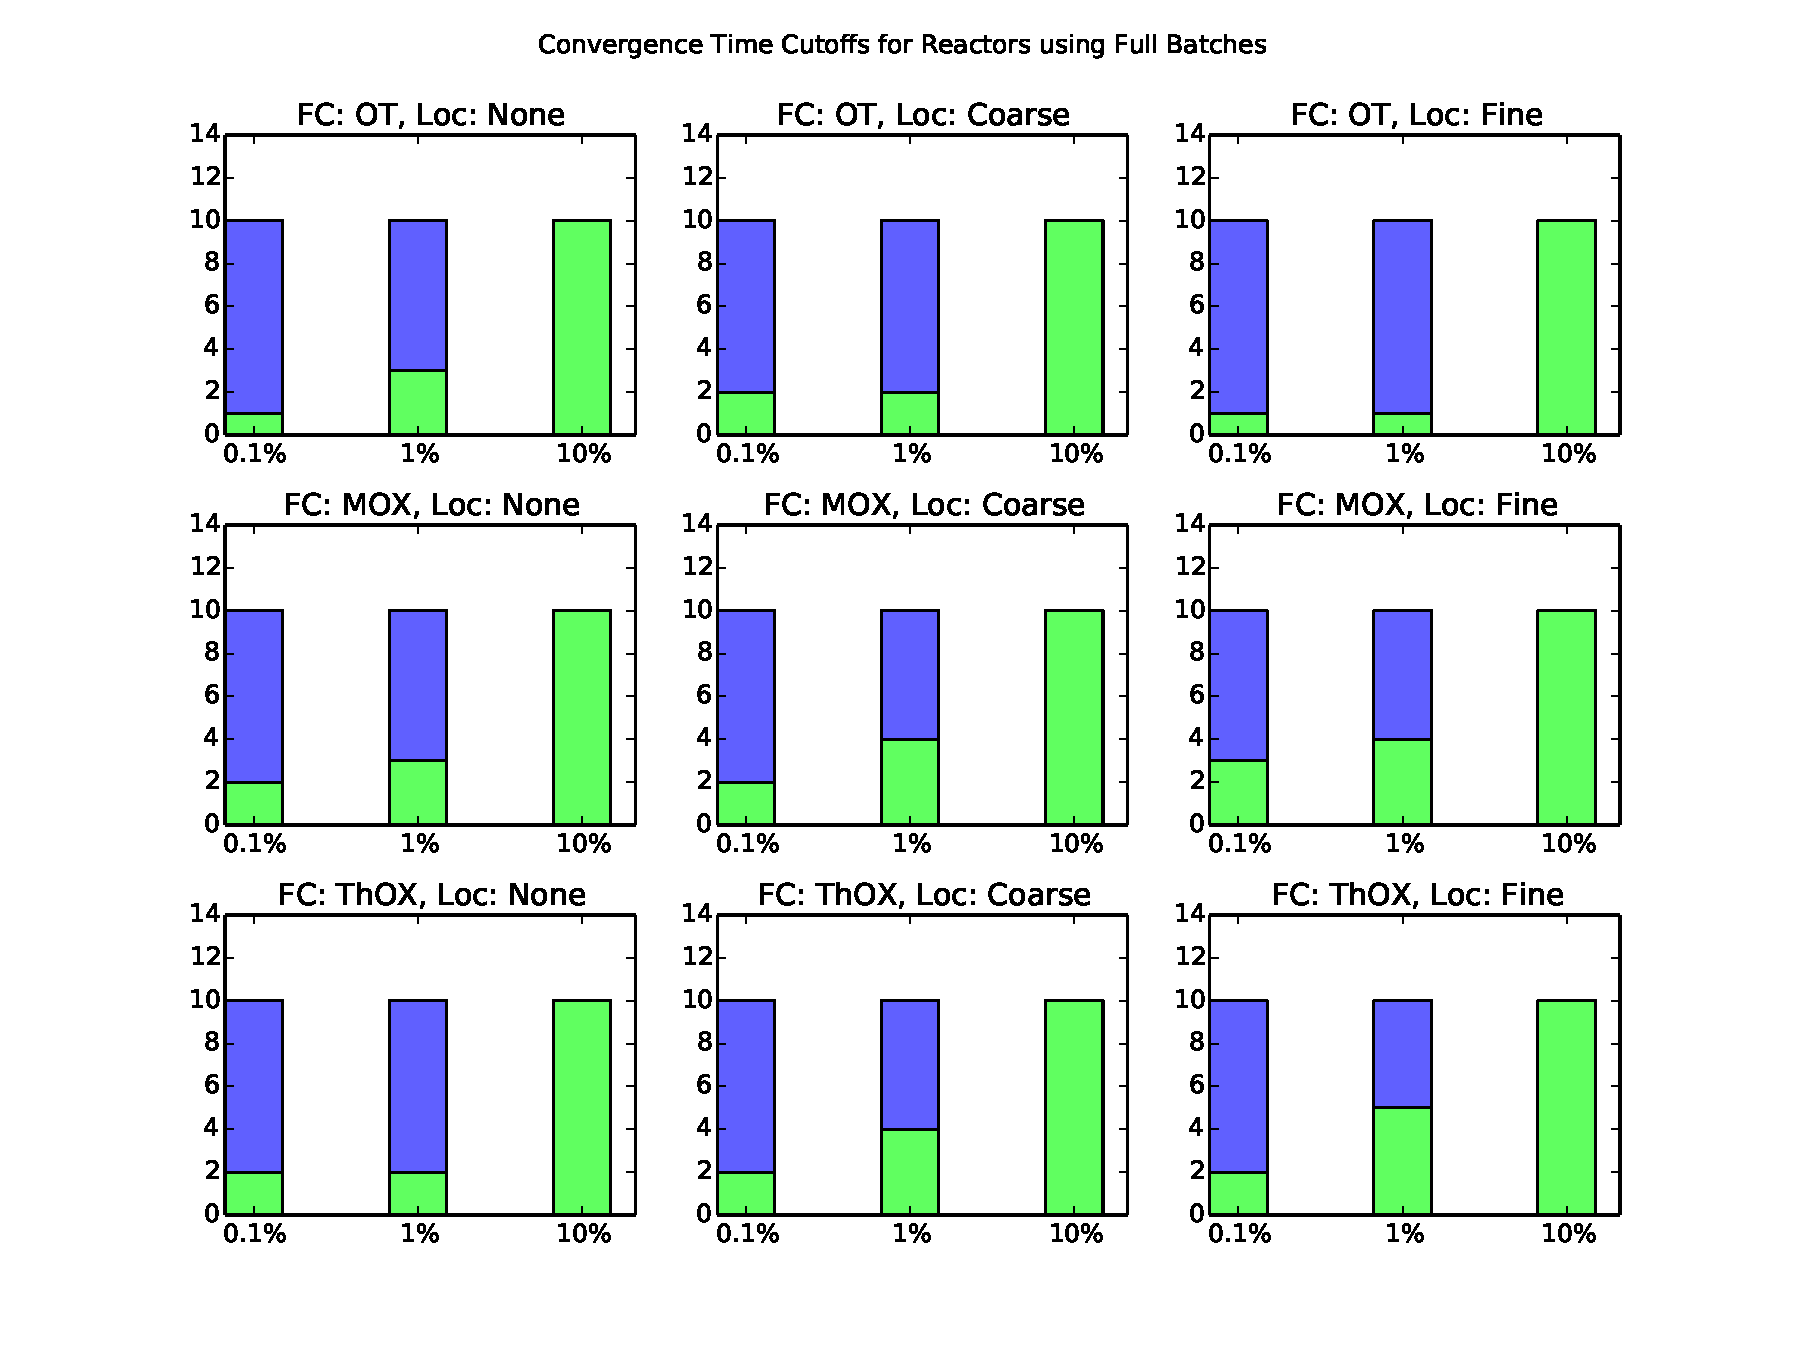
\includegraphics[width=.95\textwidth]{hist_front_rxtr_0.pdf}
    \caption[]{
      \label{fig:hist_front_rxtr_0}
      Effects of increasing convergence criteria on Front-End exchanges with
      reactors exchanging batches. Each bar is divided into how many instances
      converged (green) and did not converge (blue). }
  \end{center}
\end{figure}

\begin{figure}[h!]
  \begin{center}
    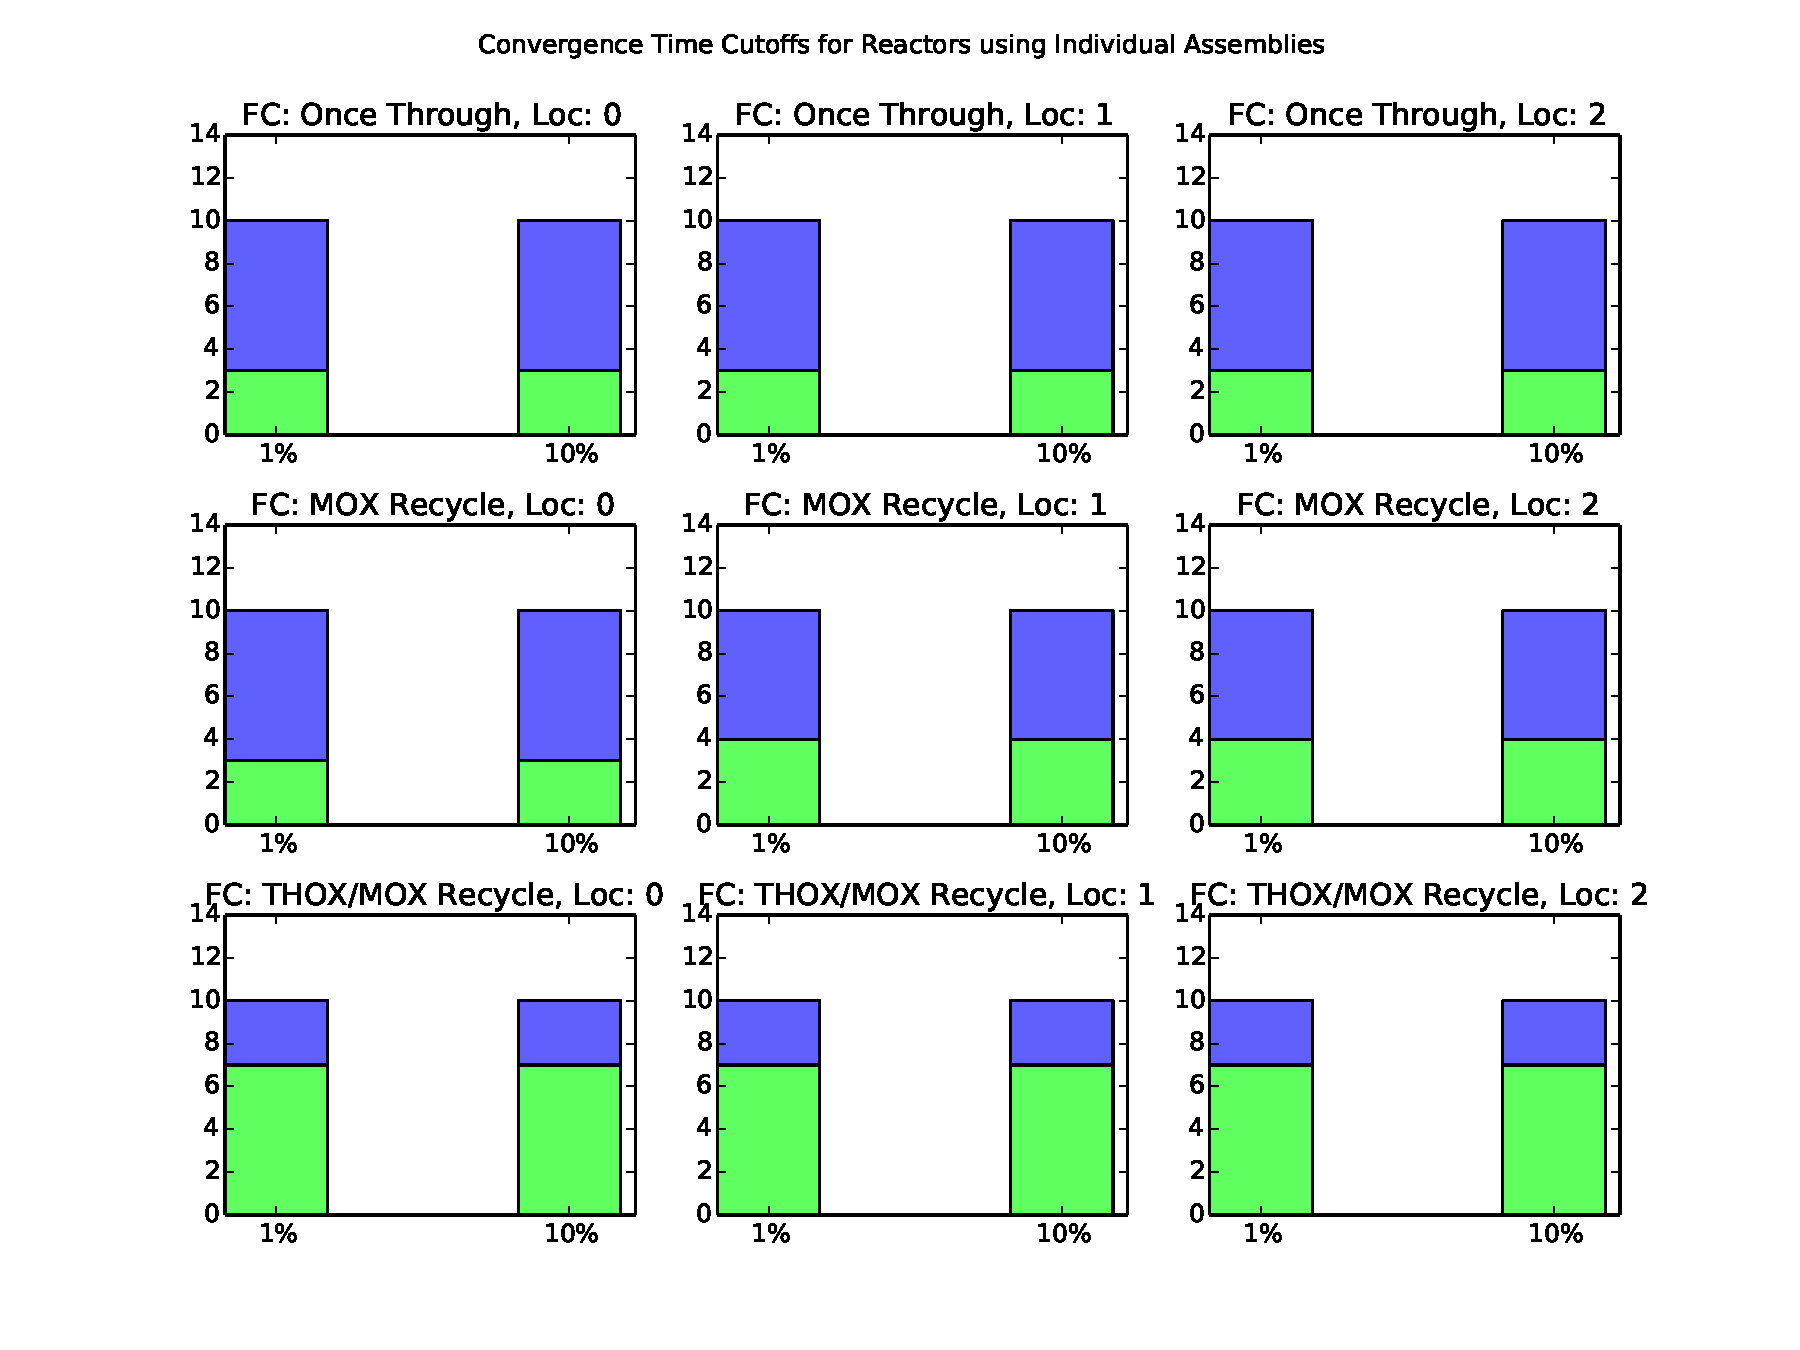
\includegraphics[width=.95\textwidth]{hist_front_rxtr_1.pdf}
    \caption[]{
      \label{fig:hist_front_rxtr_1}
      Effects of increasing convergence criteria on Front-End exchanges with
      reactors exchanging assemblies. Each bar is divided into how many instances
      converged (green) and did not converge (blue).}
  \end{center}
\end{figure}

Increasing the convergence criteria for smaller problems has a greater effect
than increasing the convergence criteria for larger problems. It is somewhat
surprising that the increase from a 1\% relative bound gap to a 10\% gap allows
full convergence in the smaller case and has no effect in the larger
case. Considering the discussion in \S \ref{sec:res:scale:front:soln}, it is
likely that the large convergence effect is due increasing the ``noise'' effect
of actual arcs. However, some speed ups in solution times are expected when
relaxing convergence criteria, and those speed ups will likely be more profound
in smaller-sized problems than larger problems.

\subsection{Back-End Exchanges}

Many of the results of the back-end exchanges mirror those of the front-end
exchanges. Therefore, this section will discuss only differences between the two
cases. The fact that so many similarities exist is striking, because from a
simulation perspective, back-end exchanges are quite different than front-end
exchanges. First, a single request is made for each commodity type that can be
consumed by support facilities. Therefore, many less requests exist in the
system. Next, the supply of used fuel is known. The total number of arcs in the
system is similar, however, as can be seen in Figure
\ref{fig:base_back_n_rxtr_n_arcs_fc1_greedy}. Furthermore, the arc
population also scales as the square of the number of reactors. 

\begin{figure}[h!]
  \begin{center}
    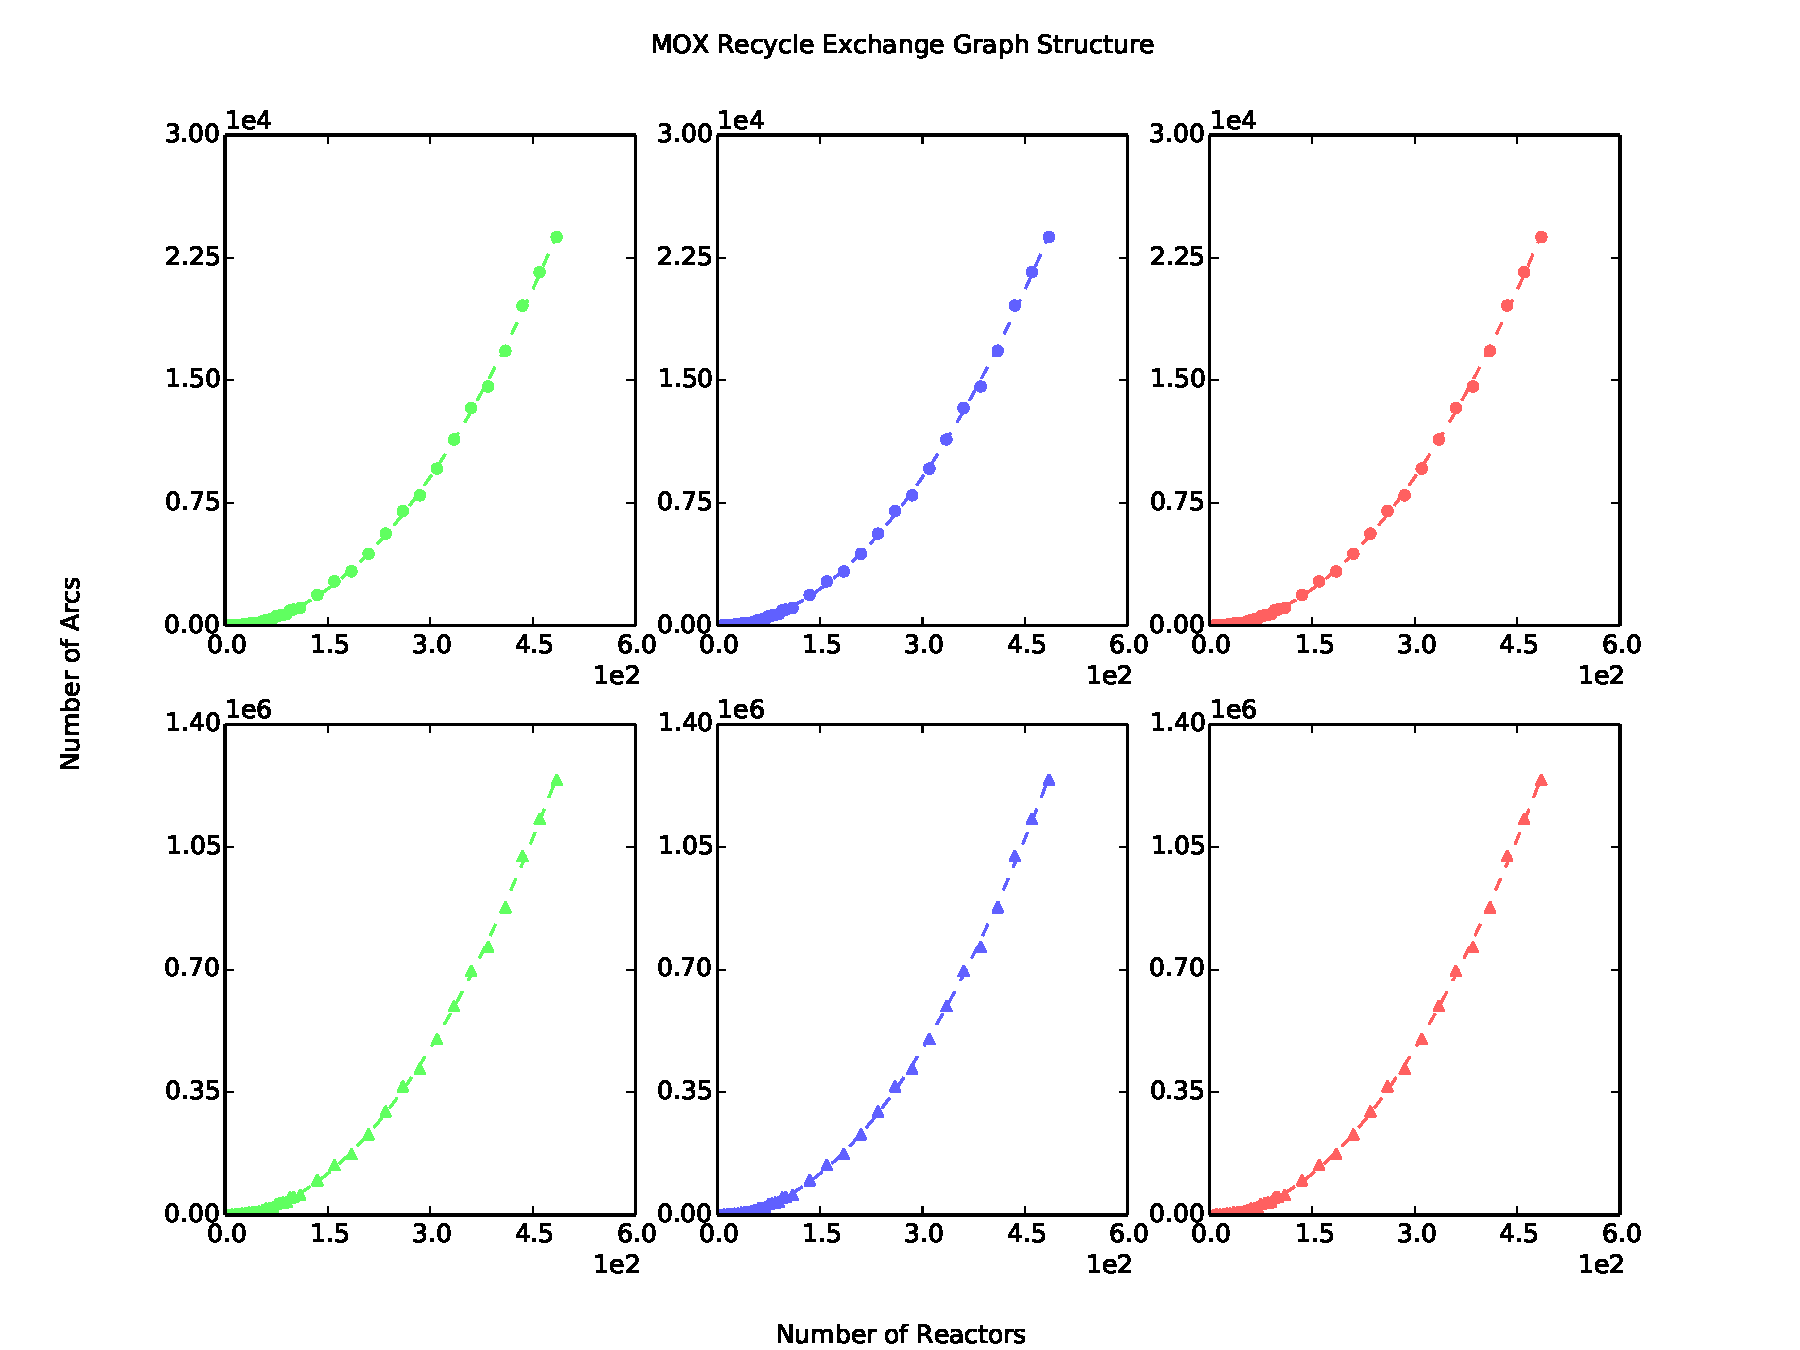
\includegraphics[width=.7\textwidth]{base_back_n_rxtr_n_arcs_fc1_greedy.pdf}
    \caption[]{
      \label{fig:base_back_n_rxtr_n_arcs_fc1_greedy}
      Arc population scaling with the number of reactors with corresponding linear fits.}
  \end{center}
\end{figure}

\subsubsection{Reference Case}

\paragraph{Greedy Solver}

The Greedy solver performs quite similarly to the front-end case. Its
performance is again linear in the number of arcs. An example of the MOX fuel
cycle is shown in Figure \ref{base_back_n_arcs_time_fc1_greedy}. As can be seen,
the linear coefficient in back-end cases is approximately twice the coefficient
of front-end cases. This observation holds irrespective of fuel cycle.

\begin{figure}[h!]
  \begin{center}
    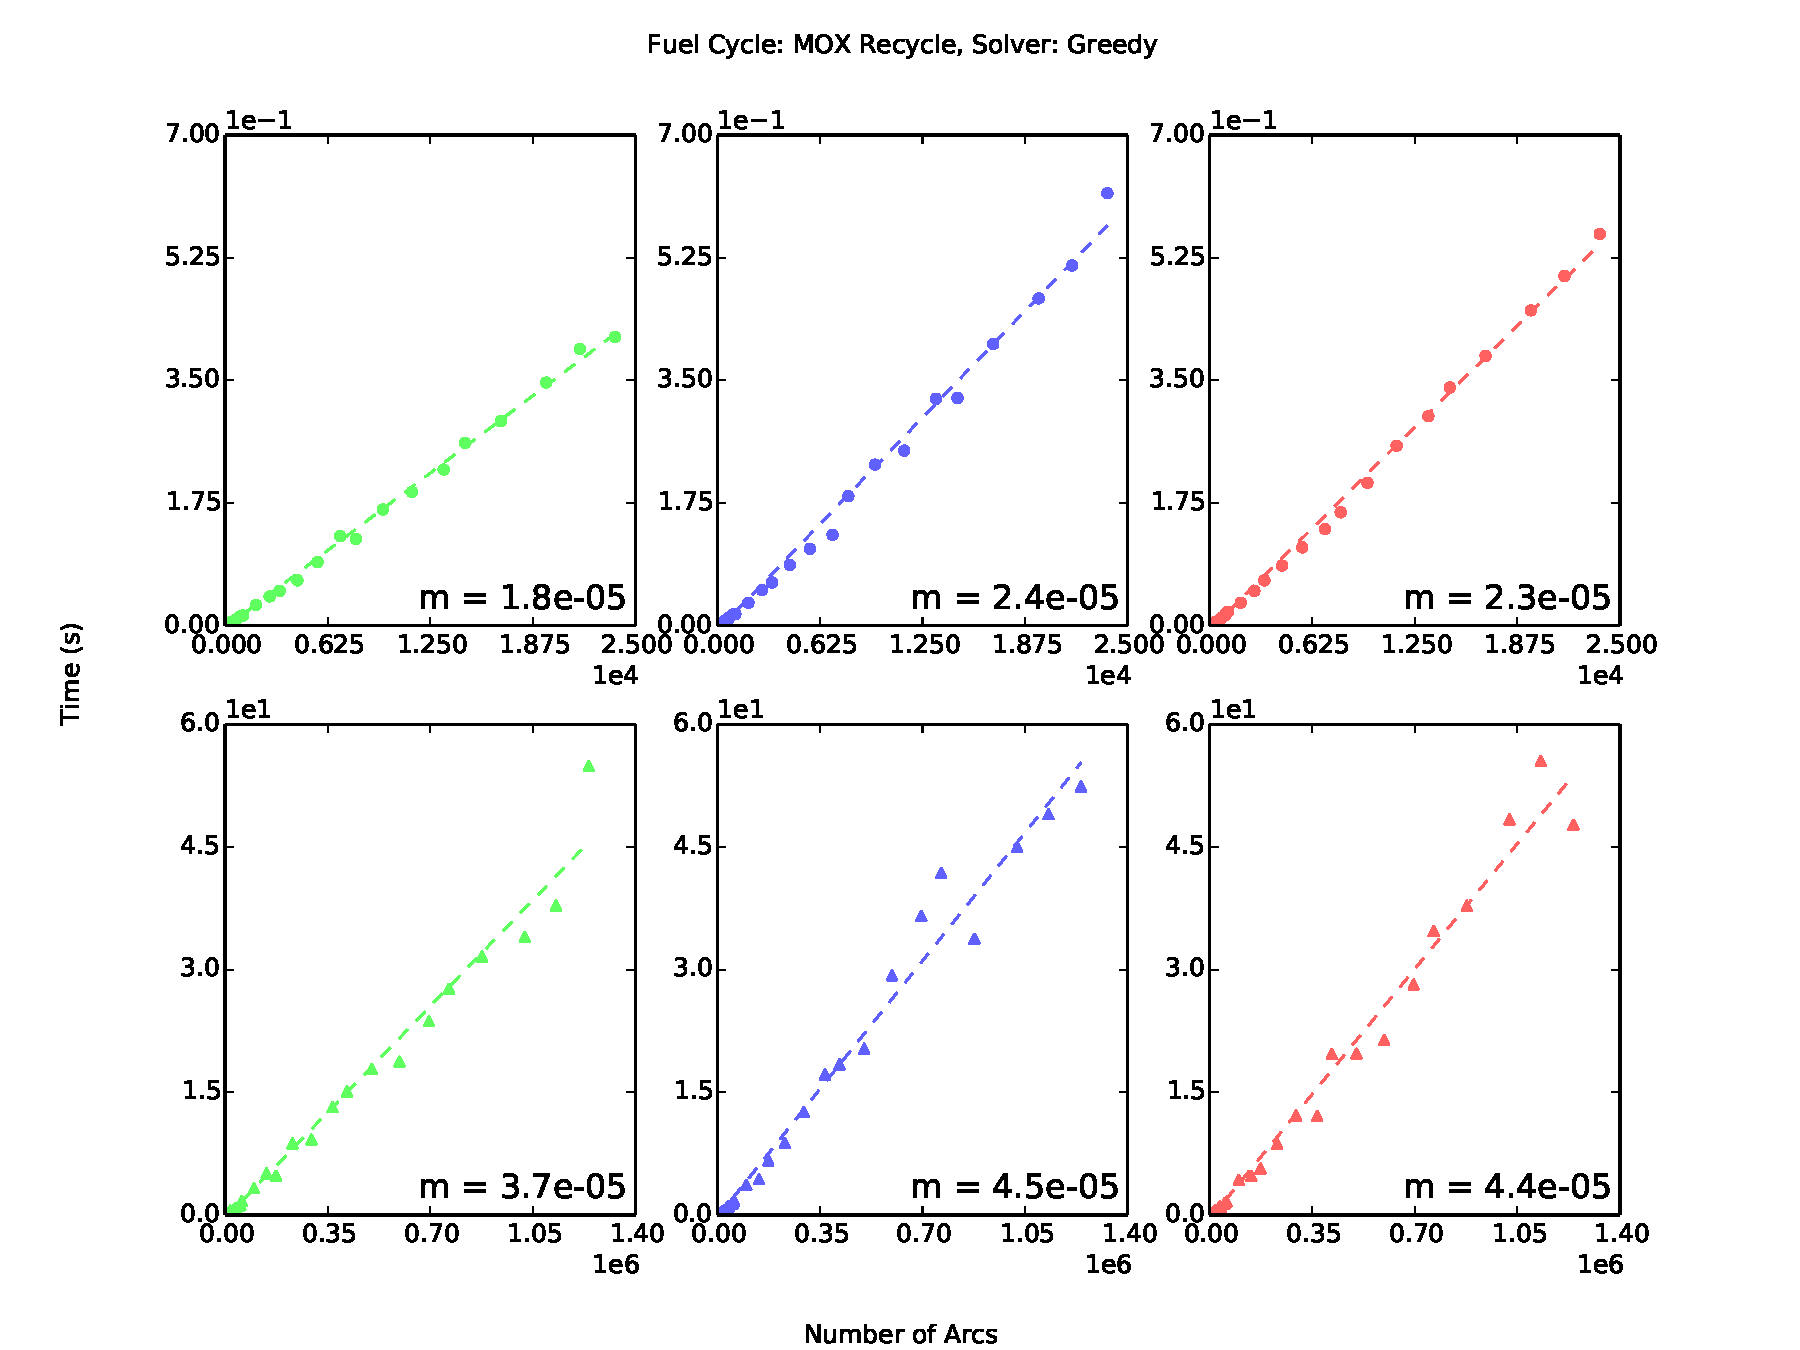
\includegraphics[width=.7\textwidth]{base_back_n_arcs_time_fc1_greedy.pdf}
    \caption[]{
      \label{fig:base_back_n_arcs_time_fc1_greedy}
      Greedy Solver results for the MOX fuel cycle as the number of arcs
      increases.      
    }
  \end{center}
\end{figure}

\paragraph{CLP Solver}

The CLP solver also performs similarly to the front-end case, as shown in Figure
\ref{fig:base_back_n_arcs_time_fc1_clp}. While the batch-based cases show linear
behavior with a slightly larger linear coefficient, the assembly-based cases
include outliers that are considerably less performant. Additionally, it is
interesting that as the fidelity of objective coefficients increases, general
solution time increases. This effectively reduces problem degeneracy, increasing
the possible objective function values.

\begin{figure}[h!]
  \begin{center}
    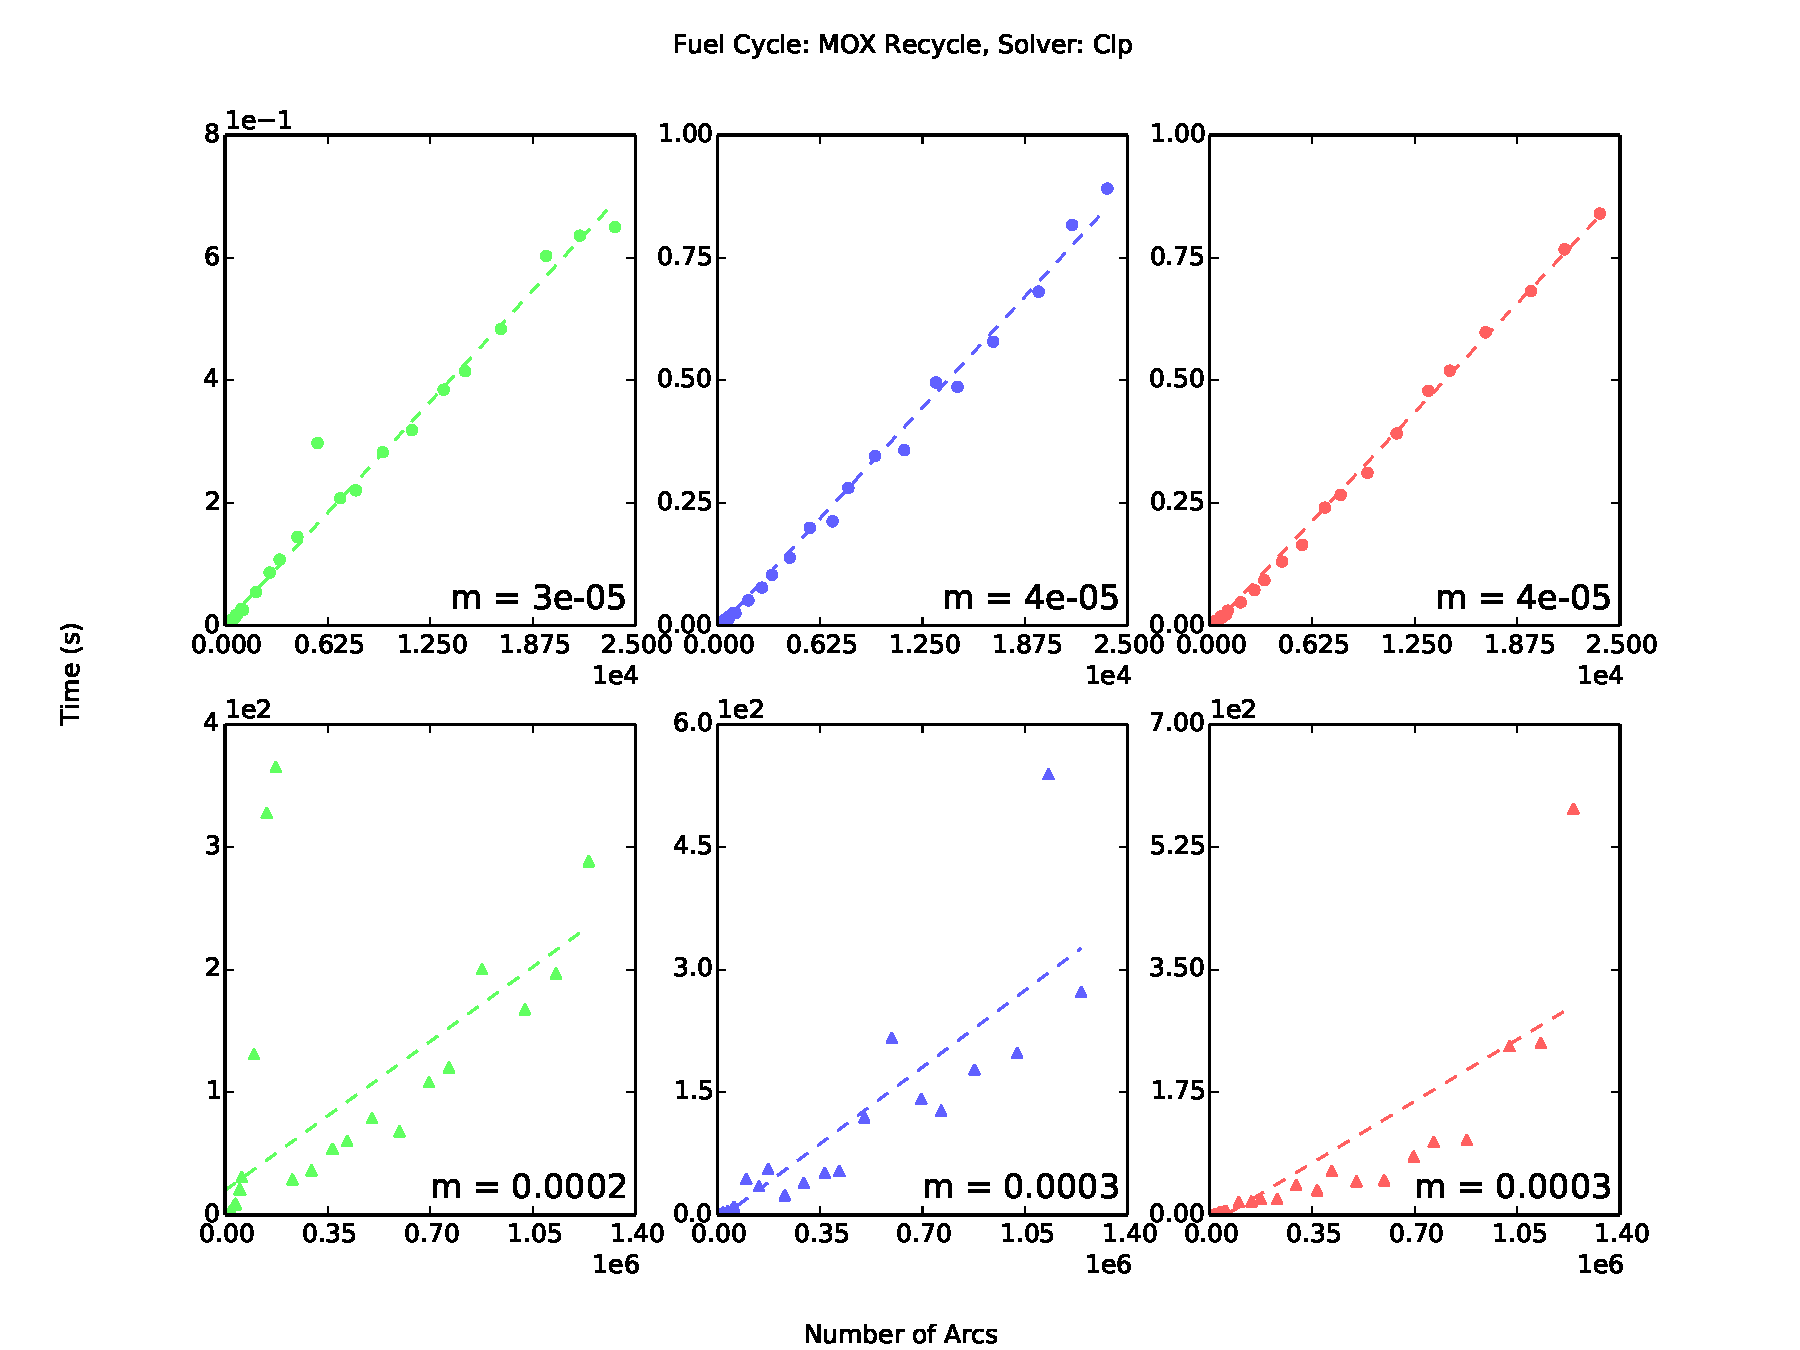
\includegraphics[width=.7\textwidth]{base_back_n_arcs_time_fc1_clp.pdf}
    \caption[]{
      \label{fig:base_back_n_arcs_time_fc1_clp}
      Clp Solver results for the MOX fuel cycle as the number of arcs
      increases.      
    }
  \end{center}
\end{figure}

\paragraph{CBC Solver}

CBC behavior is also similar to the front-end case. Importantly, exponential
scaling with problem size is again apparent, as can be seen in Figure
\ref{base_back_n_arcs_time_fc1_cbc}. The primary difference between the two
exchange types is the increased population of converged solutions for
high-fidelity reactor instances. Whereas reactor fidelity was not a large factor
with respect to convergence probability in front-end exchanges, it appears to be
a large factor for back-end exchanges.
 
\begin{figure}[h!]
  \begin{center}
    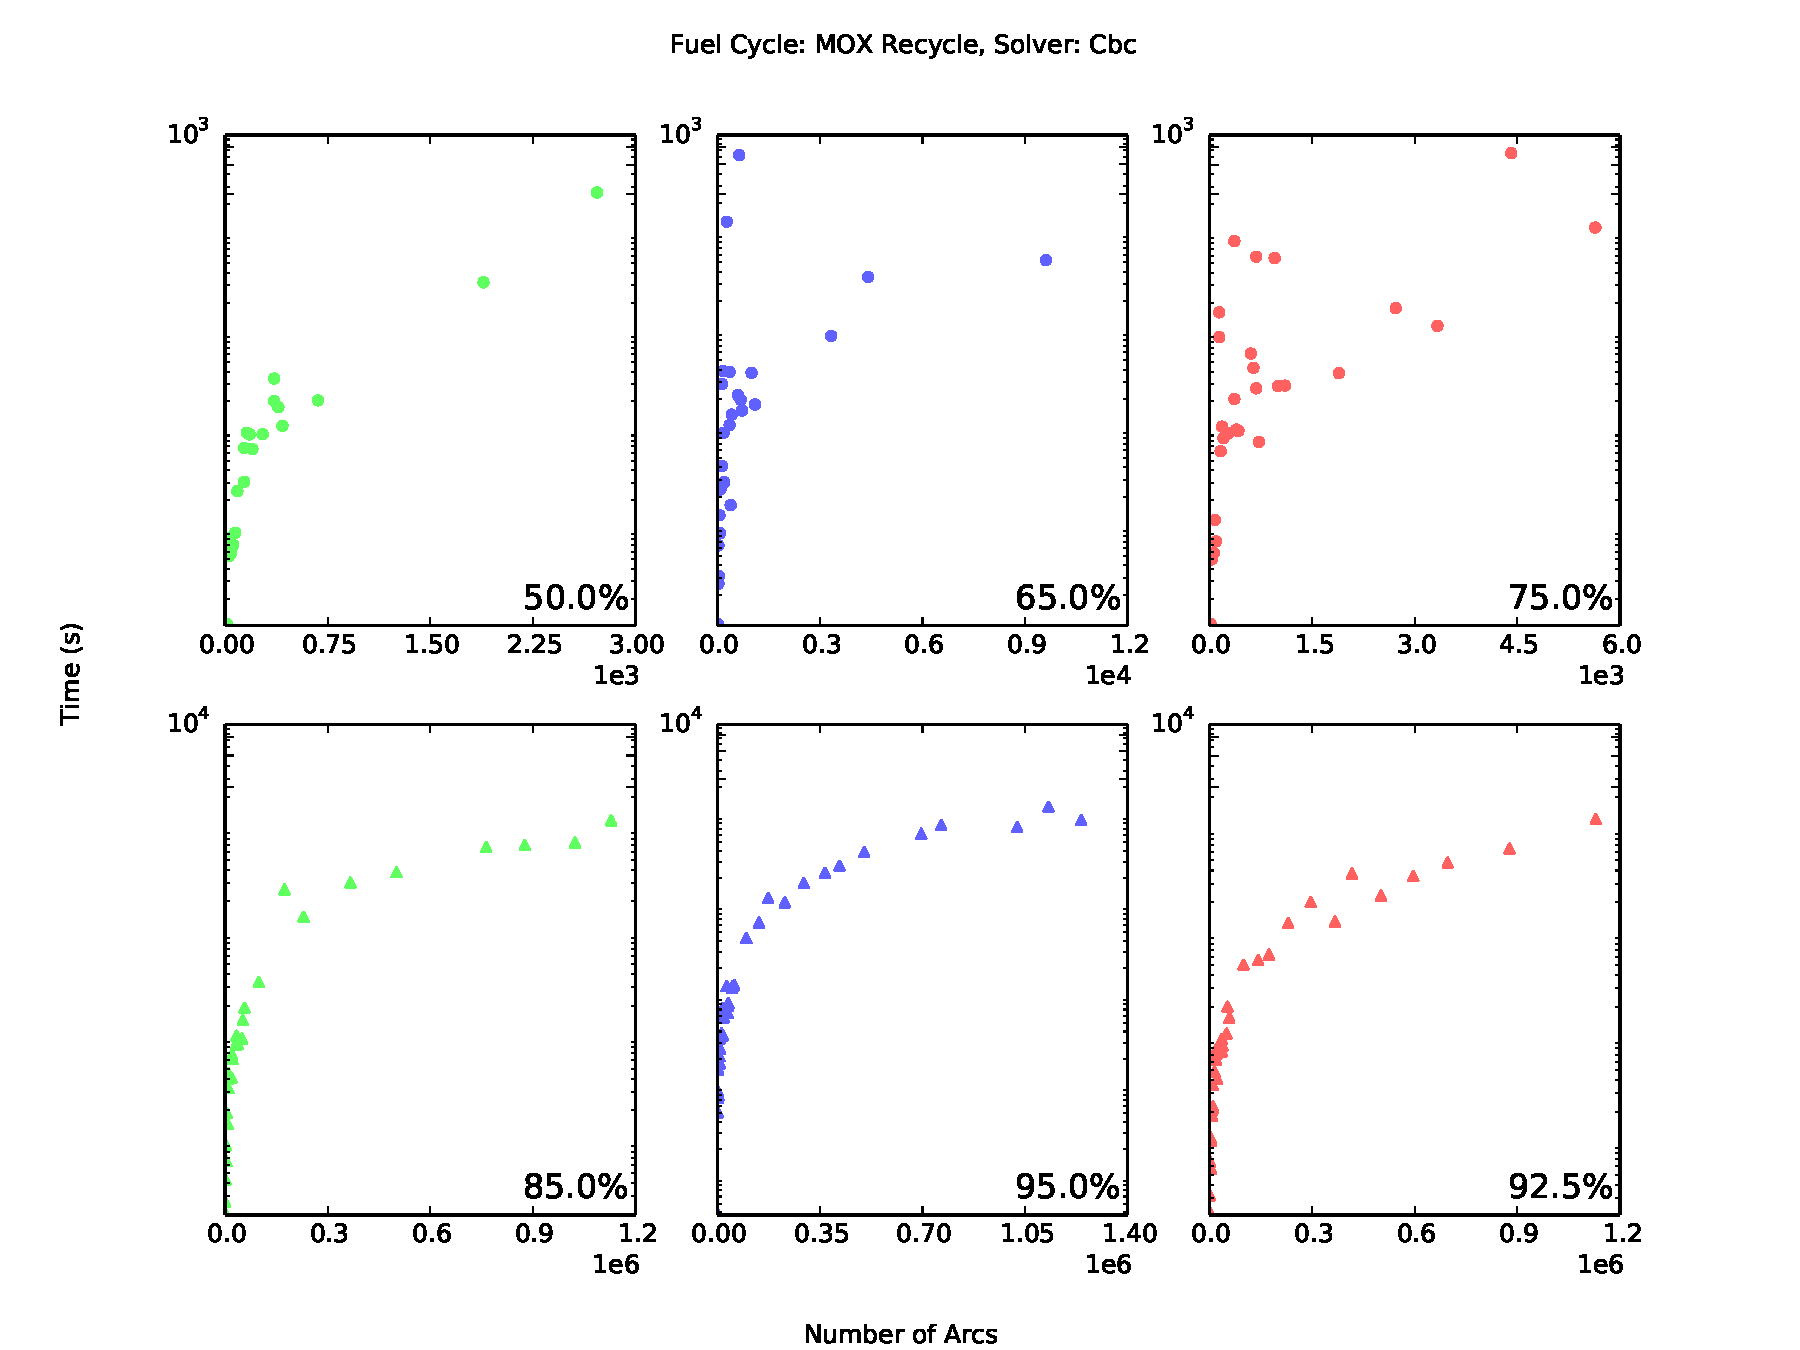
\includegraphics[width=.7\textwidth]{base_back_n_arcs_time_fc1_cbc.pdf}
    \caption[]{
      \label{fig:base_back_n_arcs_time_fc1_clp}
      Cbc Solver results for the MOX fuel cycle as the number of arcs
      increases.      
    }
  \end{center}
\end{figure}

\subsubsection{Solution Comparison}\label{sec:res:scale:front:soln}

Two notable features can be seen when comparing Greedy and CBC solutions in
Figure \ref{fig:compare_cbc_greedy_pref_flow_back_n_rxtr__fc1_}. The first is
that CBC almost always performs better than Greedy in preference space. Further,
$z^*_{\text{sim}} \leq z_{\text{sim}, \text{Greedy}}$ is true only for very
small exchanges. Additionally, CBC preference space results relative to the
Greedy solver are, in general, better for low-fidelity reactor exchanges than
high-fidelity exchanges.

Secondly, the simulation-objective gain from using CBC appears to be
problem-size independent when there are a large number of variables in back-end
exchanges. As can be seen high-fidelity reactor results in Figure
\ref{fig:compare_cbc_greedy_pref_flow_back_n_rxtr__fc1_}, when the number of
reactors is large, a relative gain in simulation objective of 30\%-40\% is
realized by using CBC. The final value is a function of the degree to which
location-based preferences are used.

\begin{figure}[h!]
  \begin{center}
    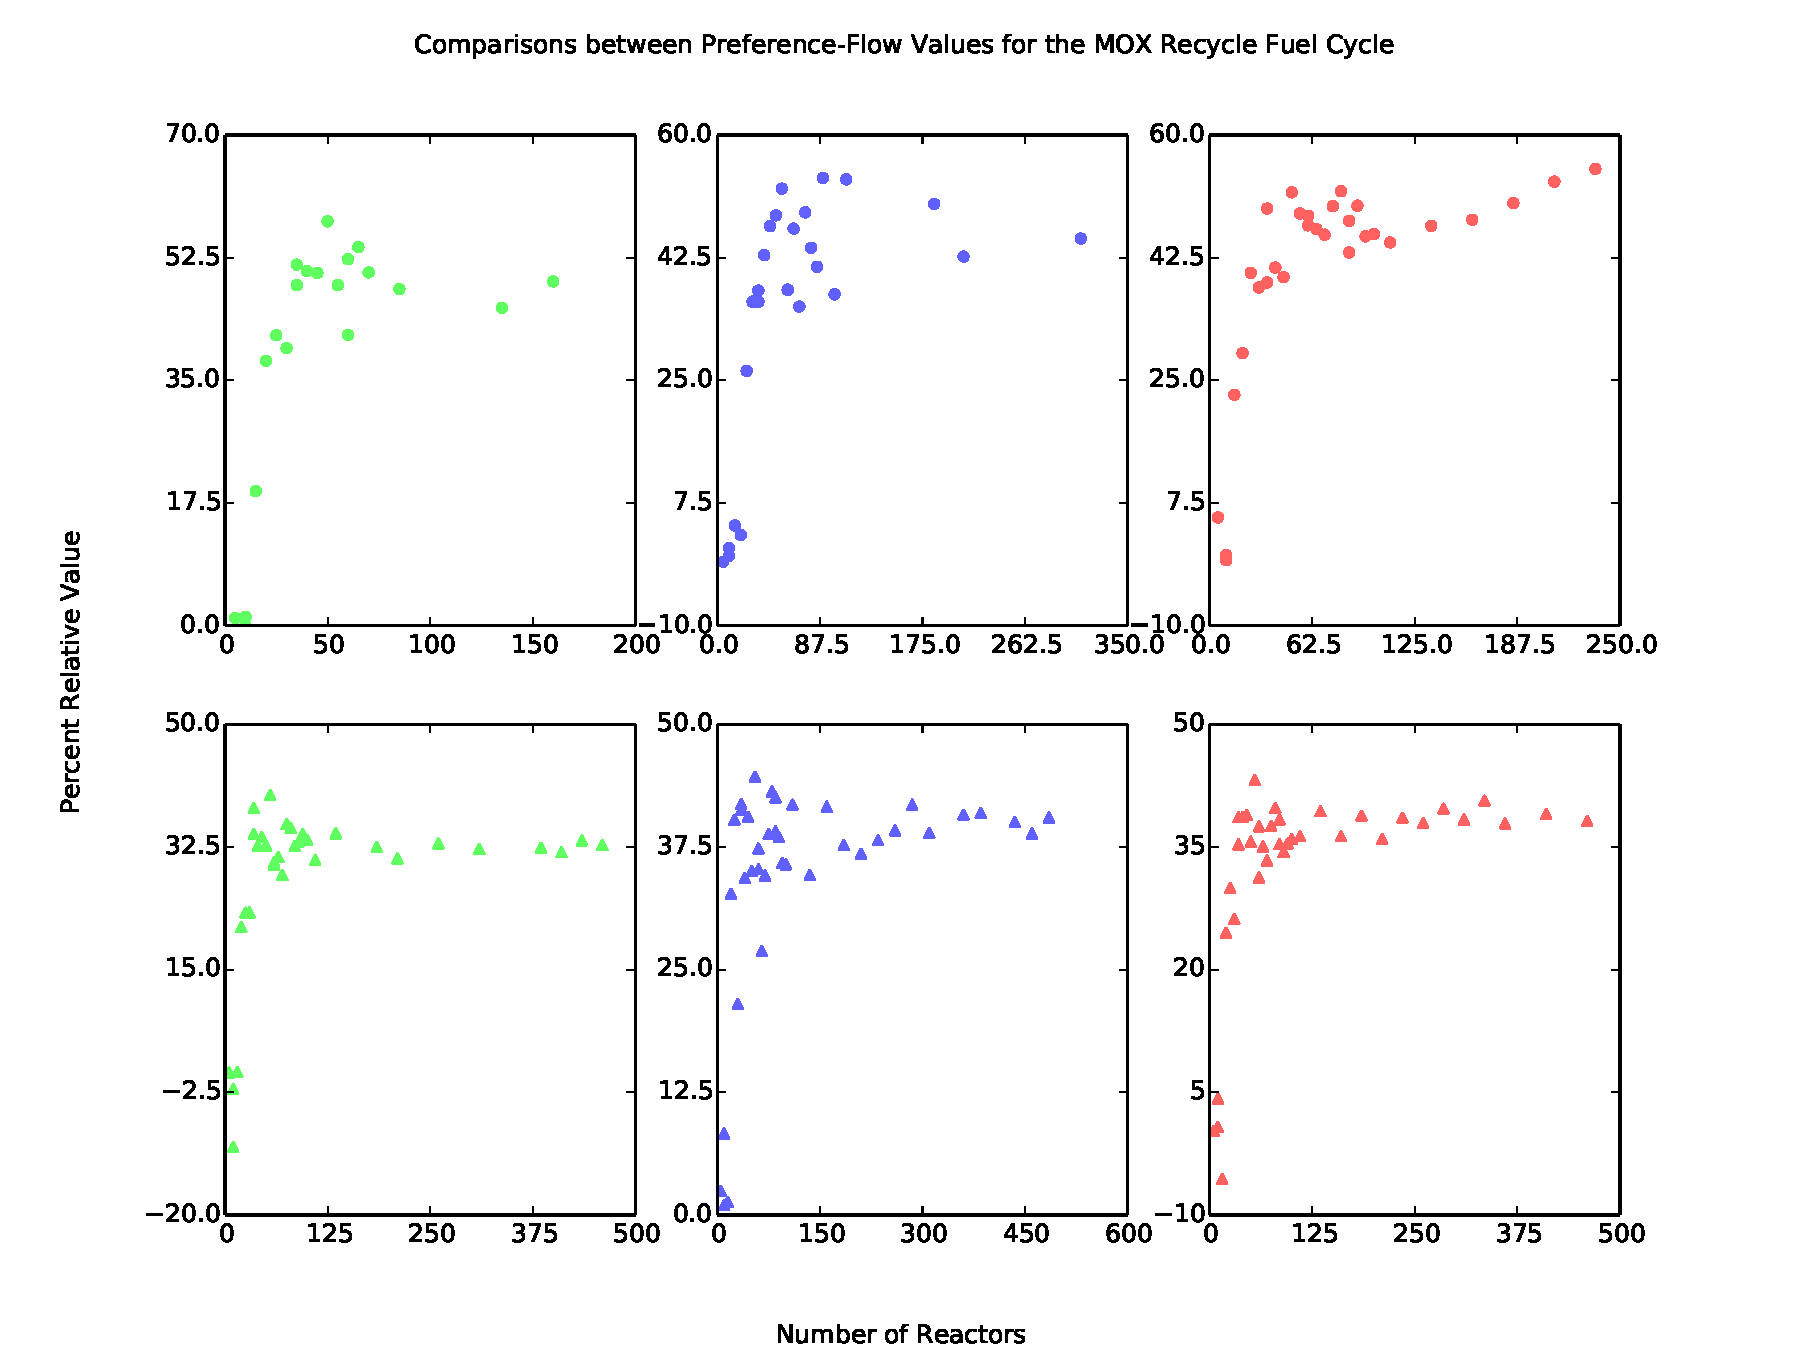
\includegraphics[width=.7\textwidth]{compare_cbc_greedy_pref_flow_back_n_rxtr__fc1_.pdf}
    \caption[]{
      \label{fig:compare_cbc_greedy_pref_flow_back_n_rxtr__fc1_}
      Comparisons between relative simulation metrics between the CBC solver and
      the Greedy solver for MOX fuel cycles. Only converged CBC
      solutions are compared.  }
  \end{center}
\end{figure}
